\documentclass[11pt]{article}
% \documentclass[letterpaper, 10 pt, conference]{ieeeconf}
\usepackage{verbatim}
\usepackage{multirow}
\usepackage{fullpage}
\usepackage{booktabs}
\usepackage{listings}
\usepackage{color}

\newcommand{\truncateit}[1]{\truncate{0.8\textwidth}{#1}}
\newcommand{\scititle}[1]{\title[\truncateit{#1}]{#1}}
\providecommand{\keywords}[1]{\textbf{\textit{Keywords: }} #1}

\usepackage[affil-it]{authblk}
\usepackage{graphicx}
\usepackage{tabularx}
\usepackage[space]{grffile}
\usepackage{setspace}
\usepackage{latexsym}
\usepackage{amsfonts,amssymb}
\usepackage{mathtools}

\usepackage{url}
\usepackage{hyperref}
\usepackage[utf8]{inputenc}

\usepackage[square,sort,comma,numbers]{natbib}
% \usepackage{natbib}

\hypersetup{colorlinks=false,pdfborder={0 0 0}}
\usepackage{textcomp}
\usepackage{longtable}

\usepackage[english]{babel}
\usepackage[autostyle]{csquotes}

\usepackage[affil-it]{authblk}

\usepackage{algorithm}
\usepackage[noend]{algpseudocode}

\usepackage{subcaption}

\usepackage{booktabs}
\begin{document}

\title{\LARGE Deep Neural Network Architectures in the Financial Industry}
\author{Henri M.B van den Bulk}
\affil{Division of Computer Science, Colorado School of Mines}
\date{\today}
\maketitle
\begin{center}
Ph.D. Qualifying Exam Report
\end{center}

% \release{0.3}     % release version; this is used to define the \version macro

% – an overview of all the machine learning topics you investigated for your project, – a literature review (e.g., list of papers identified, brief summary of each paper,
% and details on how the paper is related to your project), – details on the project’s goals and your designed study,
% – discussion of any interesting results, and
% – appropriate conclusions.

\begin{abstract}
% no more than 300 words
% no more than 300 words
In recent years the use of Deep Neural Networks (DNN) has become more prevalent and significant research has been done in this area. DNNs have different architectures to solve different Machine Learning (ML) problems. Breakthroughs in this field have been made due to the availability of data, and the ability to process a large amount of data. Datasets used in the financial industry leverage a wealth of time-series data. For each dataset classical statistical approaches have been used to interpret the data, or make predictions. These classical methods have not been able to address the multidimensionality of the data and had to rely on different approaches to correlate data.
In this research, we compare a set of DNN architectures and their fit for use in the Financial Industry.
\end{abstract}
\keywords{deep neural network, machine learning, financial industry}

\section{Introduction} \label{sec:introduction}
% What's the problem?
The financial industry (FI) has a large variety and size of data that is being used for different purposes. The FI is using data to help make recommendations, advise, or determine risk. This data includes high dimensional time-series data. For each dataset, classical approaches have been used to interpret the data, or make predictions. FI time-series data by itself can be very unpredictable as many factors can cause volatility. Many examples are relevant, such as in stock markets news articles, dividend, economic, or political events. This non-linear multidimensional data makes it a challenge for a human, or through statistical means to predict. In this research, we will leverage stock market time-series data to build our evaluation.

% Financial prediction problems – such as those presented in designing and pricing
% securities, constructing portfolios, and risk management – often involve large data sets with
% complex data interactions that currently are difficult or impossible to specify in a full economic
% model. Applying deep learning methods to these problems can produce more useful results
% than standard methods in finance. In particular, deep learning can detect and exploit interactions
% in the data that are, at least currently, invisible to any existing financial economic theory

In recent years the use of neural networks (NN) has become more prevalent and significant research has been done. NNs have been around for a long time; however, breakthroughs in this field have been made due to the availability of data. Google researchers \citet{Halevy2009TheData} published a paper showing how data could be ``unreasonably effective'' across many AI domains. With more data research has shown that NNs are capable of improving their ability to recognize patterns, and generalize those into a model.

Data is becoming more enriched through having breadth and depth of data. The combination of rich data and NN has led to the concept of deep learning (DL). With DL, researchers have created many different NN architectures to solve specific problems. NNs allow for higher order features to be discovered when more connected layers are created. An example of a DNN is convolutional neural networks (CNN) which is mainly used for vision. Vision within a biological system goes through multiple layers that help recognize higher order features, e.g. going from pixels to outlines, and finally recognizing objects.

The use of NNs and layers allows for different network graph architectures to be created. In the context of financial time-series dataset, the goal of this research is to determine which NN architectures are beneficial in this domain. Different NN architectures will be researched to discover signals and perform predictions. In the ML taxonomy, DL is under the supervised category. The use of DL architectures will be limited to this domain's problems that use supervised solutions.

% Our hypothesis is that due to the high dimensionality in FI time-series data NN have an advantage in learning higher order features.
Our work contributes by evaluating which NN architectures performs best for FI high dimensional time-series. This will provide the FI a guide on how these NN work, and leverage the architecture efficiencies with predictions.

The remainder of this paper is organized as follows. Section \ref{sec:background} provides the needed background on deep leaning, deep neural network architectures, financial industry multidimensional time-series, the experimentation environment (lab), and the deep neural networks that are under evaluation. In Section \ref{sec:experiments}, we lay out the different experiments that will be conducted, and what specific questions we try to answer to determine which architecture performs the best. In the final Section \ref{sec:conclusion}, we conclude our findings.

% Layout the structure of this article
% Why is it a problem?
% What are we going to look at?

\section{Background and Related Work} \label{sec:background}

The goal of this section is to provide a background on FI datasets, what other researchers have done, and which NNs we will be evaluating. In addition, we will layout how we use an experimentation environment for conducting the experiments in.

\subsection{Financial Industry} \label{sec:financial-industry}

The FI is a broad categorization that focuses on providing financial services to businesses and consumers. These services range from money management, wealth management, banking, credit card processing, insurance option, brokerage services, or investment function. Within these service domains prediction models, which we will call models moving forward, their purpose is to help investors with portfolio recommendations, pricing equities, equity or index pricing, risk management, and marketing. Research by \citet{Leigh2002ForecastingSupport} demonstrates that using NN for equity pricing is beneficial when looking at price history and volume history. Additionally, an exhaustive amount of research in this domain is well described in a survey paper by \citet{Bahrammirzaee2010ASystems}.

Within the industry, specific models have been developed for specific purposes. For example, the risk tolerance model (RTM) is used to determine the tolerance an individual might have to changes in the market. These models take in limited static data and do not adapt to changes of those individuals. A core reason for this is that the variety of data and possible significant correlated data is high as pointed out by \citet{Heaton2016DeepFinance}. As a result, these models are subject to over-fitting or poor at predicting. They propose using DL to deal with the high dimensionality of the complex features and allow to expand the model to include additional relevant features, which is a key property of DL.

This property of DL is key to being able to leverage it for high dimensional problem spaces, such as stock market predictions. We will be examining different dimensions in financial time-series data. Specifically, we will focus on stock market predictions.

% re-examined EMH, and leverage other perspectives of the Socionomic Theory of Finance (STF), behavioral economics, and behavioral finance as described by \citet{Bollen2011TwitterMarket}. We will be examining different dimensions in financial time-series data, specifically we will focus on stock market predictions.
% Reference: Apply DL to Enhance Momentum Strategies

\subsubsection{Stock Market Prediction}
% rewrite the following sentence
While most research in DL considers tasks that are easy for humans to accomplish, predicting stock returns using publicly available information is notoriously difficult, even for professional investors given the high level of noise in stock price movements. Ideally, the stock price correctly reflects the market's valuation of the security. The noise in stock's price can come from many sources, such as corporate actions, world events, or the behavior of emotional investors.

In the world of stock market predictions, there are many outcomes on which a model can focus. We already mentioned stock return, where a model will be optimized around a differential in a stock price. To be clear, within the industry a stock is a type of security that per contract indicates an ownership in a corporation or/and represents a claim on part of the corporation's assets and earnings. This is also called the common stock, versus a marketable security like exchange traded fund (ETF). A marketable security can track a commodity (e.g. gold or grain), an index (Standard and Poor 500), bonds, or a collection of assets. Either a marketable stock or common stock(security) trade like a common stock on a stock exchange.

Stock market predictions have been of interest to businesses and academia. In the business world, there are algorithmic trading companies that focus on building models to beat the odds in the market. According to the effective market hypothesis (EMH) \citet{10.2307/2350752,JOFI:JOFI518} the market is efficient, i.e. the stock prices reflect all events. EMH states that present and historical stock prices are not indicators of the future price of a stock, rather the price is driven by new information. The new information can be a variety of data such as news, corporate actions, or analyst reports. The researchers stated that news is unpredictable, and as such the stock market is based on a random walk \cite{doi:10.2469/faj.v51.n1.1861}. Consequentially, a stock market prediction cannot exceed fifty (50) percent accuracy, due to it being a random walk.

% This implies that when  that the use of news events as a correlation to stock prices could be leveraged as an indication of stock price.
EMH's assumption is that events are reflected in the stock price, as such that would imply that these events can be signals to a stock price when correlation can be found. This has allowed other research to re-examined EMH, and leverage other perspectives of the socioeconomic theory of finance (STF), behavioral economics, and behavioral finance as described by \citet{Bollen2011TwitterMarket}.

To enable looking at the different events, those events need to be turned into quantifiable features. In the case of news events, the content needs to be munched into a vector space so that DL techniques can leverage them. This is an area where different natural language processing (NLP) techniques can be leveraged to interpret the historical news. NLP is used to extract features from articles, such as bags-of-words, noun phrases, and named entities.
These features can be represented as vectors of real numbers using word embeddings. A popular way of doing this is using Word2Vec \citet{Mikolov2013EfficientSpace}. Figure \ref{fig:nlp-example} shows an example how a sentence is deconstruction using embedding. The example is from using Google's NLP API, where a sentence is provided, and the DL algorithm can now make syntactical sense of what it has been provided. These DLs are core to personal assistants like Siri, Amazon Alexa, and Google Assistant.

Embedding provides a way to perform syntactic parsing and allow for sentiment analysis. For extracting a structured representation of the event, \citet{Ding2015} demonstrate using open information extraction (Open IE) to generate tuples that represent the actor, action, and object of the event. These tuples are then fed into a convolutional neural network (CNN) to generate daily predictions of the stock price. They demonstrate in the research that by reducing the text to tuples the core essence of a financial news article can be ascertained.

\begin{figure}[!ht]
	\centering
	\makebox[\textwidth]{
    	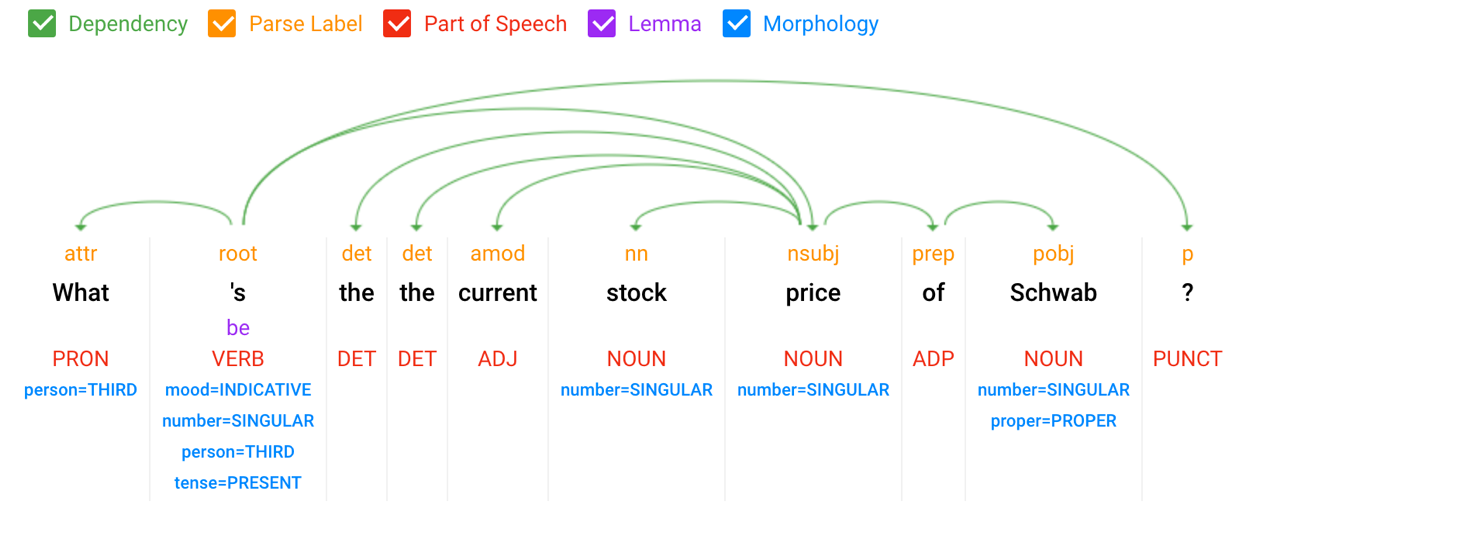
\includegraphics[
        width=\paperwidth,
        height=10cm,
		keepaspectratio]{media/nlp-example}}
	\caption{Google's Natural Language Processing}
	\label{fig:nlp-example}
\end{figure}
Public sentiment is shown to make an impact on the stock market as well. \citet{Bollen2011TwitterMarket} demonstrate that by using social media data from Twitter and performing different sentiment analysis techniques, they are able to predict changes in various economic and commercial indicators. They found that they could predict with an accuracy of 86.7\% the daily up and down changes in the closing values of the DJIA. The approach used here was a classification of up and down of the next day's closing price of a stock.
% and can not be predicted based on historical prices
% that present and historical stock prices are not indicators of the future price of a stock, rather the price is driven by new information.
% As mentioned, according to EHM the market is efficient, i.e. the stock prices reflects all events and can not be predicted based on historical prices. This implies that when  that the use of news events as a correlation to stock prices could be leveraged as an indication of stock price.

% Early approaches to predicting stock market where based on the Effective Market Hypothesis (EMH) \citet{10.2307/2350752,JOFI:JOFI518}. EMH stated that present and historical stock prices are not indicators of the future price of a stock, rather the price is driven by new information. New information can be a variety of data such as news. The researches stated that news is unpredictable, and as such the stock market is based on a random walk  \citet{doi:10.2469/faj.v51.n1.1861}. With this random behavior a stock market prediction can not exceed fifty (50) percent. Their fundamental assumption is that the price of a stock reflects all know information, and the price movement is in response to news or other events.
Some specific research has focused on using DL to predict stock indexes by \citet{Heaton2016DeepFinance}. Stock indexes are a composite indicator of a hypothetical portfolio of securities representing a market or a related segment. The Standard and Poor (S\&P) 500 and the US Aggregate Bond Index are common benchmarks for the American stock and bond markets, respectively. As an investor, you can not invest directly in an index, rather investments can be made on derivatives of an index in the form of a mutual fund that mimics the portfolio of investments.

Their approach is interesting in that an index like the S\&P 500 is based on 500 underlying securities. By defining this as a hierarchical structure, that is represented as layers in a DNN with a single output value, where the DNN can learn the complex interaction between the data.

The research compares the use of deep auto-encoder and long short-term memory networks to predict the single output value in a non-linear manner.
% we obtain a deep feature policy (DFP) which for every combination of inputs tells us which corresponding action gives us the best approximation of the target variable.  In the above picture, we see the  setup  for  a  DFP  which  through  two  hidden  layers  approximates  the  S\&P500  based  on  the  ten  largest  companies
% In particular DL can detect and exploit interactions in data that are invisible to any existing financial economic theory.
%http://www.investopedia.com/articles/technical/081501.asp

Investors leverage stock price charts to gain a visual insight into movement predictions. Looking for movement is officially called a price momentum trading strategy, where momentum is the measurement of the velocity of price changes. To determine the underlying features of the price velocity, i.e. isolate the indicators, different approaches require the engineering of features from historical data. After the underlying features are determined, they are then leveraged to look for significant movement in a direction.

An example of using this strategy occurred when investors jumped on the movement for Netflix in 2013. Between January and October, the stock surged 260\%, because investors jumped on the uptrend, in essence more capital moving into the stock. \citet{Takeuchi2013ApplyingStocks} layout an approach of using a feed forward neural network (FFNN) to discover the underlying features. They leveraged an auto-encoder composed of stacked restricted Boltzmann machines (RBMs) to extract features from stock prices. Even though their model only had an accuracy of about  53.36\%, they were able to get a return of 45.93\% on an annualized basis.

In stock market predictions, what is important to understand is that a specific strategy albeit having good features for prediction other features should be taken into account. This multidimensionality problem is ideal for DL where many different features, through embedding, can be applied without having to stay with a single strategy. Existing financial economic theory tends to focus on a specific set of features; however, DNNs can detect and exploit interactions in data that might be invisible.
% "Market momentum is measured by continually taking price differences for a fixed time interval. To construct a 10-day momentum line, simply subtract the closing price 10 days ago from the last closing price. This positive or negative value is then plotted around a zero line. The formula for momentum is:
% M = V - Vx
% Where V is the latest price, Vx is the closing price x number of days ago."

% Momentum traders look for stocks moving significantly in one direction on high volume and try to jump on board to ride the momentum train to a desired profit. For example, Netflix (Nasdaq:NFLX) surged over 260\% to \$330 from January to October in 2013, which was way above its valuation. Its P/E ratio was above 400, while its competitors' were below 20. The price went up so high primarily because many momentum traders were trying to profit from the uptrend,
% We use an autoencoder composed of stacked restricted  Boltzmann  machines  to  extract features from the history of individual stock prices
% Considering the pervasive use of historical price charts by investors and noting that the primary mode of anal-ysis is visual, we take an approach similar to that used by Hinton and Salakhutdinov (2006 ) to classify hand-written  digits.   In  particular,  we  use  an  autoencoder composed  of  stacked  restricted  Boltzmann  machines (RBMs)  to  extract  features  from  stock  prices,  which we then pass to a feedforward neural network (FFNN)

%Attrition data

% Beeline word2vec

% \subsubsection{Financial Modeling} \label{sec:fin-modeling}

% Google Domestic Trends
% Shows search trends in specific areas

% Rewording needed
% Should highlight that other dimension help with the underlying sentiment
% A growing body of research has however critically examined EMH[31] , in particular from the perspective of the Socionomic Theory of Finance (STF)[42,41], behavioral economics[47] and behavioral finance[36] . Numerous studies show that stock market prices do not follow a random walk and can indeed to some degree be predicted[4,24,16,43] thereby calling into question EMH’s basic assumptions. Some recent research also suggests that news may be unpredictable but that very early indicators can be extracted fromo nline social media (blogs, Twitter feeds, etc.) to predict changes in various economic and commercial indicators. This may conceivably also be the case for the stock market. For example, Gruhl et al. [18] showed how online chat activity predicts book sales.

% Why is FI time-series data high dem
% Model
% Model Building Pipeline
% Describe what's volatility in the market, volume, movement, and other indicators

% \subsubsection{Financial Model Transparency} \label{sec:financial-model-transparency}
% https://www.technologyreview.com/s/604122/the-financial-world-wants-to-open-ais-black-boxes/amp/
% 1D - Works well with high volatility not with low
% When there might be underlying patterns the LSTM will work well.

% \subsubsection{Data Problems} \label{sec:data-problems}

% Imbalanced data
% Incomplete data
% High Dimensionality

% \subsection{Symbolic Representation of Time Series} \label{sec:sax}

\subsection{Deep Neural Networks} \label{sec:dnn}
% TODO talk about that DNN are stacked Boltzmann machines...
DNN has emerged in the last half a decade as a powerful set of techniques that mimick human's perceptual abilities. DNNs represent different architectures that have been formulated as part of DL research. DL is a class of ML techniques, where many layers of processing in a hierarchical architecture are leveraged for pattern classification, and for feature or representation learning (RL). In research, DL is more recently referred to as representation learning (RL) \citet{Bengio2013RepresentationPerspectives, MAL-006}.

Artificial intelligence (AI) is the overall scientific field that has ML and DL as subfields. Figure \ref{fig:ml-history} shows the general history of AI, which originated around 1950 with Alan Turing \cite{Alan1950Turing.Intelligence} devising the ``Turing Test''. The main objective of the test was to test a machine’s ability to exhibit intelligence, indistinguishable from a human.

ML’s focus has been to devise algorithms and machines that recognize patterns in data. The algorithms and systems that learn the patterns can adapt and ultimately make predictions without the need to explicitly program the logic required to accomplish a task. By leveraging large amounts and variety of data the patterns are discovered and then used to predict outcomes. DL refines ML where the focus is for machines to automatically learn, by discovering higher order understanding, e.g. seeing an image, discovering shapes, and to identifying the shapes.

\begin{figure}[!ht]
	\centering
	\makebox[\textwidth]{
    	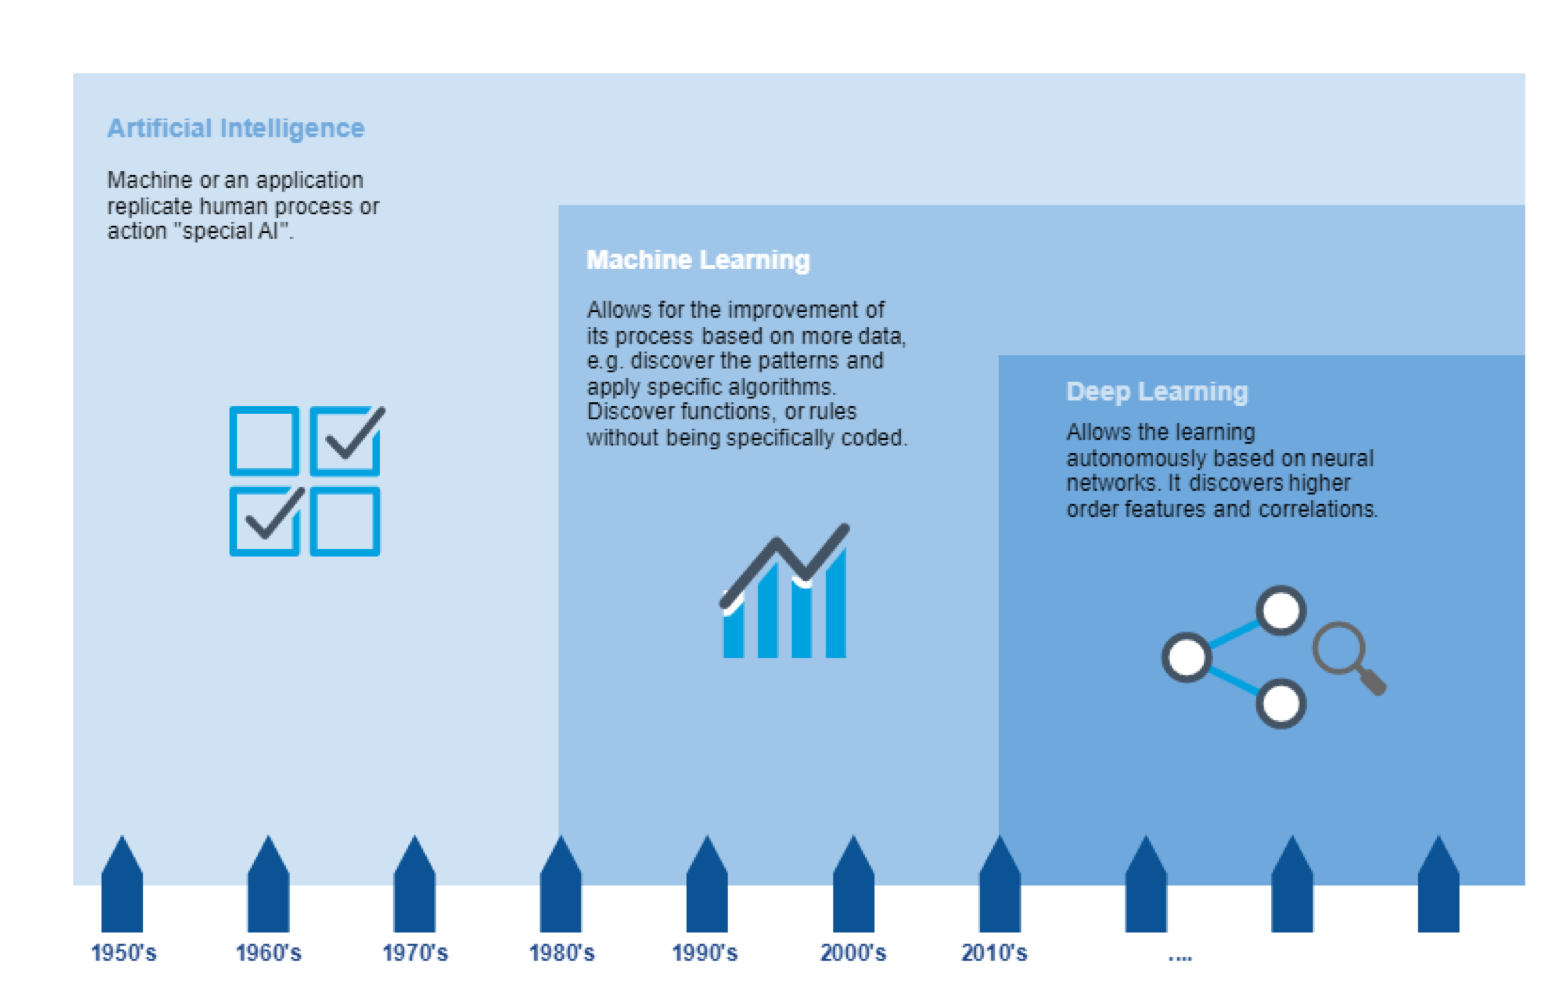
\includegraphics[
        width=\paperwidth,
        height=10cm,
		keepaspectratio]{media/ml-history}}
	\caption{Artificial Intelligence History}
	\label{fig:ml-history}
\end{figure}

NNs found their original inspiration from biology, where the term ``neural network'' can also be used for neurons in a brain, which is composed of a number of neurons. The analogy between biology and NN will we be debatable. However, it is a good cognitive representation of the model. Figure \ref{fig:biology-nn} shows the representation, where the simple NN is the perceptron which has a single neuron. The neuron has a tree structure with multiple input nodes and a single output node, each of which is connected to each other. Due to the artificial nature, the NN is typically referred to as an artificial neural network (ANN) to distinguish it from a biological neural network.
\begin{figure}[!ht]
	\centering
	\makebox[\textwidth]{
    	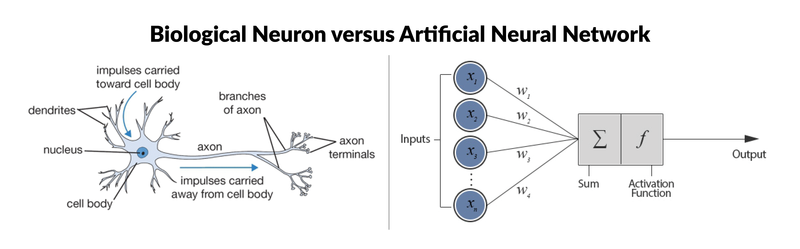
\includegraphics[
        width=\paperwidth,
        height=8cm,
		keepaspectratio]{media/content_content_neuron}}
	\caption{Biological Comparison to an Artificial Neural Network}
	\label{fig:biology-nn}
\end{figure}

Back in 1943 \citet{McCulloch1990AActivity}, for the first time, proposed a mathematical model of an individual neuron as a simple computing machine. The neuron computes a weighted sum of its inputs and outputs a single value. The neuron can be viewed as a single mathematical function \(y=\ F\left(X\right)\). The input space \textit{X} is high-dimensional which is expressed as a vector \(X=\left(x_1,...,x_n\right)\). Equation \ref{eq:sum-function}, represents the weighted sum of the inputs. If the neuron merely would output the value of the function, it would not be able to be used as a boolean function. Instead, this the function needs to produce a value between zero and one, essentially an indication of when to activate (fire) based on a threshold.

To determine the activation, each neuron has an activation function that defines when to fire, similar as in biology. As such, a neuron can be thought of as a gate. The most common activation function is the sigmoid function, which results in an ``S'' shaped curve that continues with a value between zero and one. This provides for the full Equation \ref{eq:gate-function} for the gate. A key observation here is that because of the combination of the summation and activation the unit will start to fire based on specific patterns. This is a key feature of NN where the patterns are recognized in a non-linear manner.
\begin{equation}
\label{eq:sum-function}
y=(\sum_{i=1}^n w_i*x_i)
\end{equation}

\begin{equation}
\label{eq:gate-function}
y=sigmod(\sum_{i=1}^n w_i*x_i)
\end{equation}

So far, a neuron is only activating based on its inputs, without considering the weights. The weights are used to adjust the input values to optimize for the desired output. Take, for example, that based on a set of stock features the gate needs to classify to buy or sell a given stock. To accomplish this, an objective function is used that determines the loss (cost) when making changes, also called the loss function. The changes that need to be made are to the weights. The loss function calculates the derivative with respect to the input values. The weights then get adjust to being optimal (lowest loss) to match the inputs to the desired output. The process for doing this is called the gradient descent (GD), see Figure \ref{fig:gradient-descent}. There are many approaches to calculating the loss, such as using mean square error (MSE), or cross-entropy (CE).
\begin{figure}[!ht]
	\centering
	\makebox[\textwidth]{
    	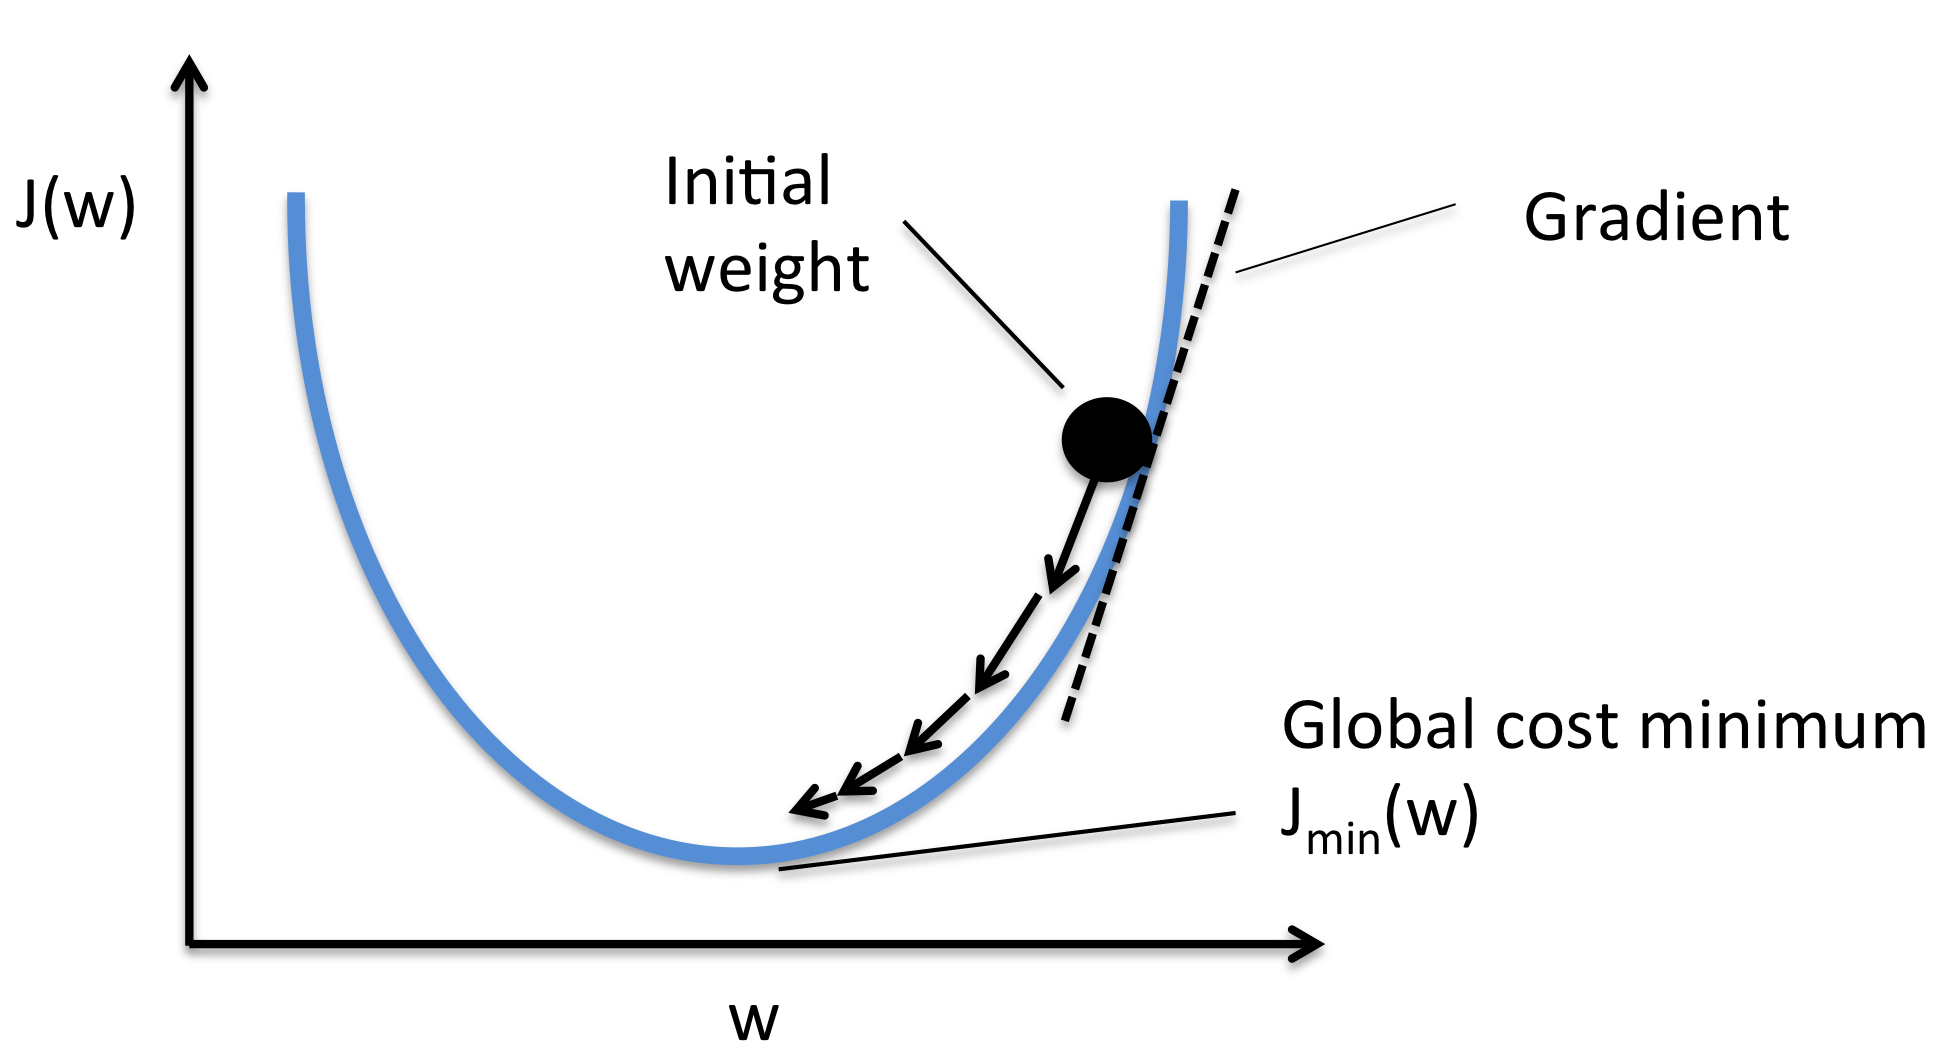
\includegraphics[
        width=\paperwidth,
        height=8cm,
		keepaspectratio]{media/gradient-descent}}
	\caption{Gradient Descent}
	\label{fig:gradient-descent}
\end{figure}

Intuitively, the updates to the weights do not happen all at once, rather GD's optimization algorithm tries to find the local minimum, e.g. lowest loss, in multiple steps. Each step that GD takes is called an \textit{epoch}, and the number of steps is a parameter expressed in \textit{epochs}. The steps are proportional to the negative (direction) of the gradient, which is called the step size.

The notion of a network comes from combining multiple gates together, similar to an electronic circuit. In ANN, the gates are completely independent of each other and from a system engineering perspective form a non-linear black box as pointed out by \citet{Prieto2016NeuralChallenges}. The manner in which an ANN is organized follows a common pattern, as shown in Figure \ref{fig:ann-diagram}.

The pattern is based on building layers of gates, where each layer is fully connected to the next layer. In general, there are three types of layers. First, there is the input layer, that based on the number of features (dimensions), has a set of gates. These gates are then connected to the next layer, called the hidden layer. This layer can have a different number of layers in itself, which each layer having different number of gates. This is called the hidden layer, as this forms the \textit{blackbox} of the ANN. The third, and final layer is the output layer. Depending on the number of variables that need to be predicted there is that number of gates in that layer. The number of layers and composition of the layers is what we call the ANN architecture.
\begin{figure}[!ht]
	\centering
	\makebox[\textwidth]{
    	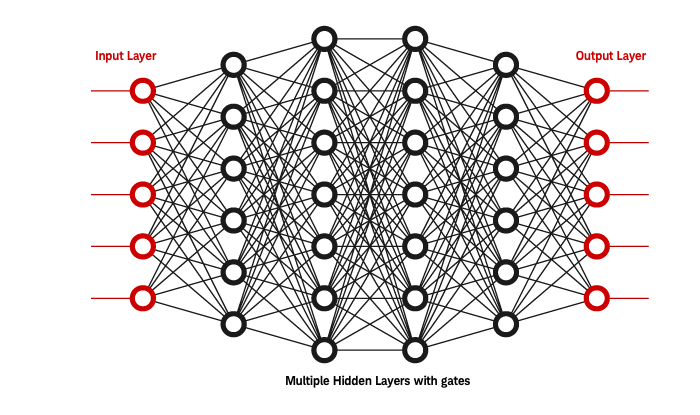
\includegraphics[
        width=\paperwidth,
        height=8cm,
		keepaspectratio]{media/ann-diagram}}
	\caption{Artificial Neural Network}
	\label{fig:ann-diagram}
\end{figure}

The original ANNs and ML algorithms, such as Guasian mixture models (GMMs) and hidden Markov models (HMMS), had shallow structured architectures. The shallowness stems from those models using typically a single layer of feature transformations. The feature, e.g. raw input of transformation was only done in specific problem spaces vs. generalizing. These models work very well in solving simple or well-constraint problems.

In more complex or higher dimensional problems these models are unable to recognize patterns. By using different ANN architectures their problems can be addressed. Due to the multiple layers, or at least two hidden layers, ANNs get the name of DNN.

% Backpropagation - Compute the partial derivative of the error with respect to each layer backwards (weights) = gradient gradient is a value with a direction (e.g. partial derivative)
With the many connected gates and layers, the DNN is capable of identifying higher order features or patterns in the input data. The way it is feeding the output of each gate to the next set of gates is called a feed forward network (FFN). The challenge with FFNs is that at each gate the gradient is determined.

The goal of DNNs, in supervised learning, is to find an \(F\left(X\right)\) that best maps a set of inputs to their correct output. As such, the gradient needs to be determined for the whole network. In the 1980s \cite{Rumelhart1985LearningPropagation} backpropagation was used to propagate the local gradient from the output back through the network to the input layer. This algorithm uses the chain rule to calculate the gradients of the network. In other words, the loss of the whole network needs to be propagated backward, so that each gate can determine its contribution to the loss. This process is called the network optimization, which as discussed earlier, can be accomplished with GD. However, other optimizers exist as well, which is beyond the scope of this paper.
%Backpropagation uses these error values to calculate the gradient of the loss function. In the second phase, this gradient is fed to the optimization method, which in turn uses it to update the weights, in an attempt to minimize the loss function.

We have been using the term gate to describe the logical unit in the DNN. As we will describe later in this paper more sophisticated DNNs have multiple operators and gates within a single logical unit. To ensure we can generalize the different types, moving forward this paper will refer to these logical units as unit.

\subsubsection{Training and Validation} \label{sec:training}
% http://neuralnetworksanddeeplearning.com/chap3.html
The part of updating the weights in a network and leveraging techniques like backpropagation is part of what is called training the model. Essentially, it is the process of providing sample (training) data with correct output values, e.g. supervised learning, then performing an optimization which propagates the loss backward. Each unit then minimizes its loss and updates its weights.

As part of training large data sets are needed, so that the network can correctly recognize the patterns in the data. In 2009, researchers \citet{Halevy2009TheData} of Google published a paper showing how data could be ``unreasonably effective'' across many AI domains. Further data research has shown that loss rates of training diminished, this can be observed in the loss curves during training. The use of large amounts of data is being used to recognize patterns. The decline of loss is correlated by allowing the pattern recognition to improve.

\begin{figure}[!ht]
	\centering
	\makebox[\textwidth]{
    	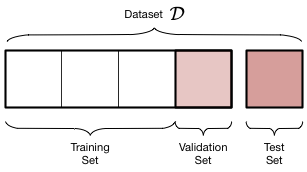
\includegraphics[
        width=\paperwidth,
        height=5cm,
		keepaspectratio]{media/train-validate-test}}
	\caption{Training data splits}
	\label{fig:train-validation-test}
\end{figure}
%https://stats.stackexchange.com/questions/19048/what-is-the-difference-between-test-set-and-validation-set

During the training, the loss and performance need to be determined. Depending on the model different metrics can be used, such as accuracy and precision for classification, or mean absolute error (MAE) for scalar models. If only the training data was to be used the model can cause overfitting, e.g. generalizing a function that perfectly fits the training data. What is really needed is for the model to generalize the patterns to make good predictions on new data. To determine if this is occurring, the data needs to be compared to a training set and new data. To enable this, the dataset \textit{D} is split as shown in Figure \ref{fig:train-validation-test}, in three sets.

The dataset \textit{D} gets split into two parts, the training, and test data. This is typically done with an 80/20 split. The test data is set aside for a final test of the performance of a fully-trained model. During the training, the training data is then split into a training set and validation set. The split, in this case, is typically 95/5. At each epoch, the loss and the metrics are calculated for these sets. This validation data set is used to compare the performances of the prediction algorithms. The MAE metric will be used to compare between the network architectures in our case.

By comparing the metrics we can see if the performance of the training set is different than the validation set. If the performance of the training set tends to be higher, the model might be overfitting. In Figure \ref{fig:metric-test-val} the difference of MAE between the training and validation can be observed. The training part, Figure \ref{train-mae}, shows that MAE is gradually minimizing; however, for the validation, this is not occurring. This is an indication that the model is starting to overfit.

To address this the model can ``punish'' the network by introducing noise. This process is called regularization, and a number of functions can be used for this, such as dropouts.

\begin{figure}
    \centering
    \begin{subfigure}[b]{0.3\textwidth}
        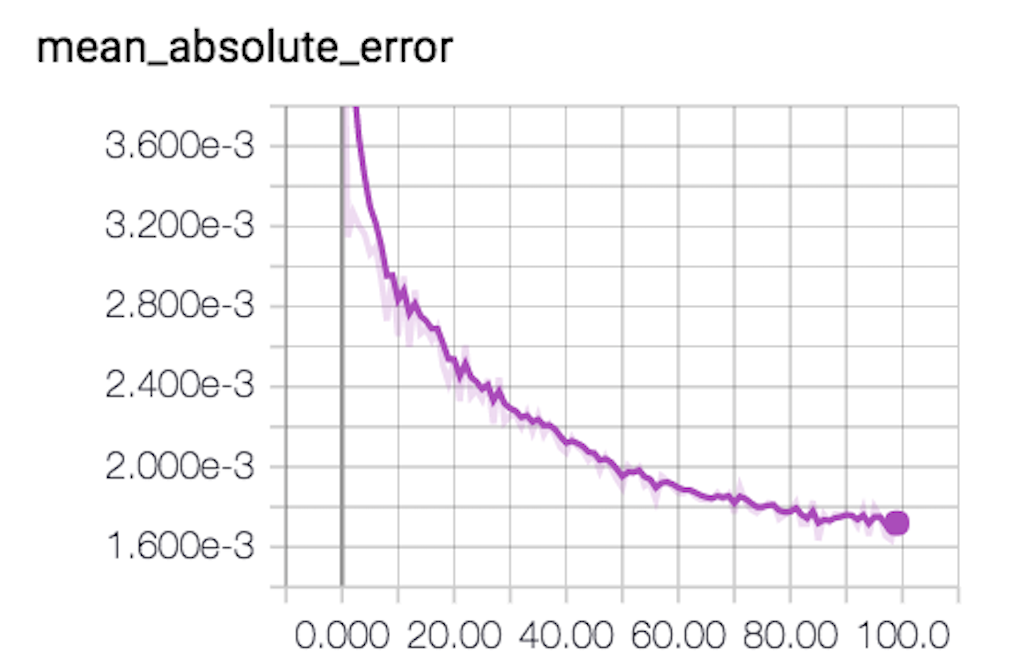
\includegraphics[width=\textwidth]{media/metric-test-val}
        \caption{Train MAE}
        \label{fig:train-mae}
    \end{subfigure}
    ~ %add desired spacing between images, e. g. ~, \quad, \qquad, \hfill etc.
    %(or a blank line to force the subfigure onto a new line)
    \begin{subfigure}[b]{0.3\textwidth}
        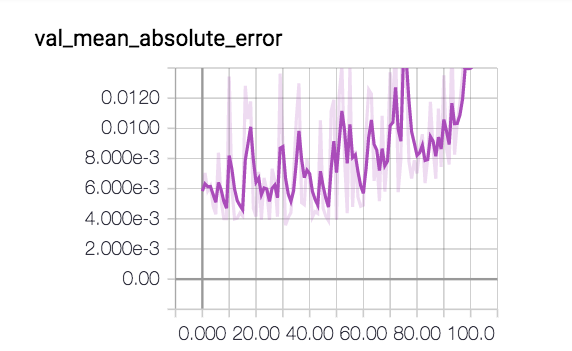
\includegraphics[width=\textwidth]{media/metric-test-val-mae}
        \caption{Validation MAE}
        \label{fig:val-mae}
    \end{subfigure}
    \caption{MAE of Train and Validation}
    \label{fig:metric-test-val}
\end{figure}


After the best model is selected the final performance is determined by using the test set of unseen values. This provides the final performance number. When different models are not being evaluated it is a valid process to skip the split of the test data.

% To deal with the overfitting you can punish complex functions and introduce noise into the neural network. Common regularization techniques to prevent this are dropout layers and punishing complex functions.

% \subsubsection{Overfitting and regularization} \label{sec:overfitting-regularization}

% Regularization is the process to reduce overfitting by forgetting training specific signals.

% \subsubsection{Hyperparamaters}
% - Hyperparameters - Batch Size, Epoc, Learning rate, etc....

% Reference: https://www.youtube.com/watch?v=qirjknNY1zo

\begin{table}[ht]
\centering
% \begin{tabular}{@{}lll@{}}
\begin{tabularx}
	{\linewidth}
%     { l l }
	{>{\hsize=.5\hsize}X>{\hsize=1.5\hsize}X}
\toprule
DNN Architecture & Description \\ \midrule
Convolutional Neural Network (CNN) & CNNs are much like FFNs, layers in the network are not fully connected to units from the previous layer. The units act as pooling (convolution), which simplify the data.\\
Recurrent Neural Network (RNN) & RNN is a fully connected network, where each units is connected to all units in the previous layer. In addition, a unit in the hidden layers has its own output with a fixed delay of one or more epochs.\\
Deep Auto-encoder (DAE) & DAE is a bottleneck structure. The network is composed of two symmetrical sides that encode and then decode the input data, in affect performing a dimensionality and noise reduction. \\
Long short-term memory (LSTM) & LSTM is a type of RNN that has memory gates that can keep track of past sequence of data. \\
Gated Recurrent Unit (GRU) & GRU is a type of RNN and has similar properties as LSTM. Its focus is being able to adaptively capture dependencies of different time scales. \\
\bottomrule
\end{tabularx}
\caption{DNN Architectures evaluated}
\label{tab:architectures}
\end{table}

\subsection{DNN Architectures} \label{sec:dnn-architectures}

As described in Section \ref{sec:dnn} the different number of layers, number of units, and connectivity create various architectures. The different architectures lend themselves to be used for different problem sets. In this section, we will explore architectures that can be applied to the financial time-series data problems.

There are many different architectures \cite{Deng2014ALearning, Schmidhuber2015DeepOverview} in DL. Research by \citet{vanVeen2017NeuralInstitute} provides a comprehensive visual representation of the architecture landscape, as shown in Figure \ref{fig:neural-networks}. For the purpose of our problem set, Table \ref{tab:architectures} summarizes the DNN architectures that we will be evaluating.

\begin{figure}[!ht]
	\centering
	\makebox[\textwidth]{
    	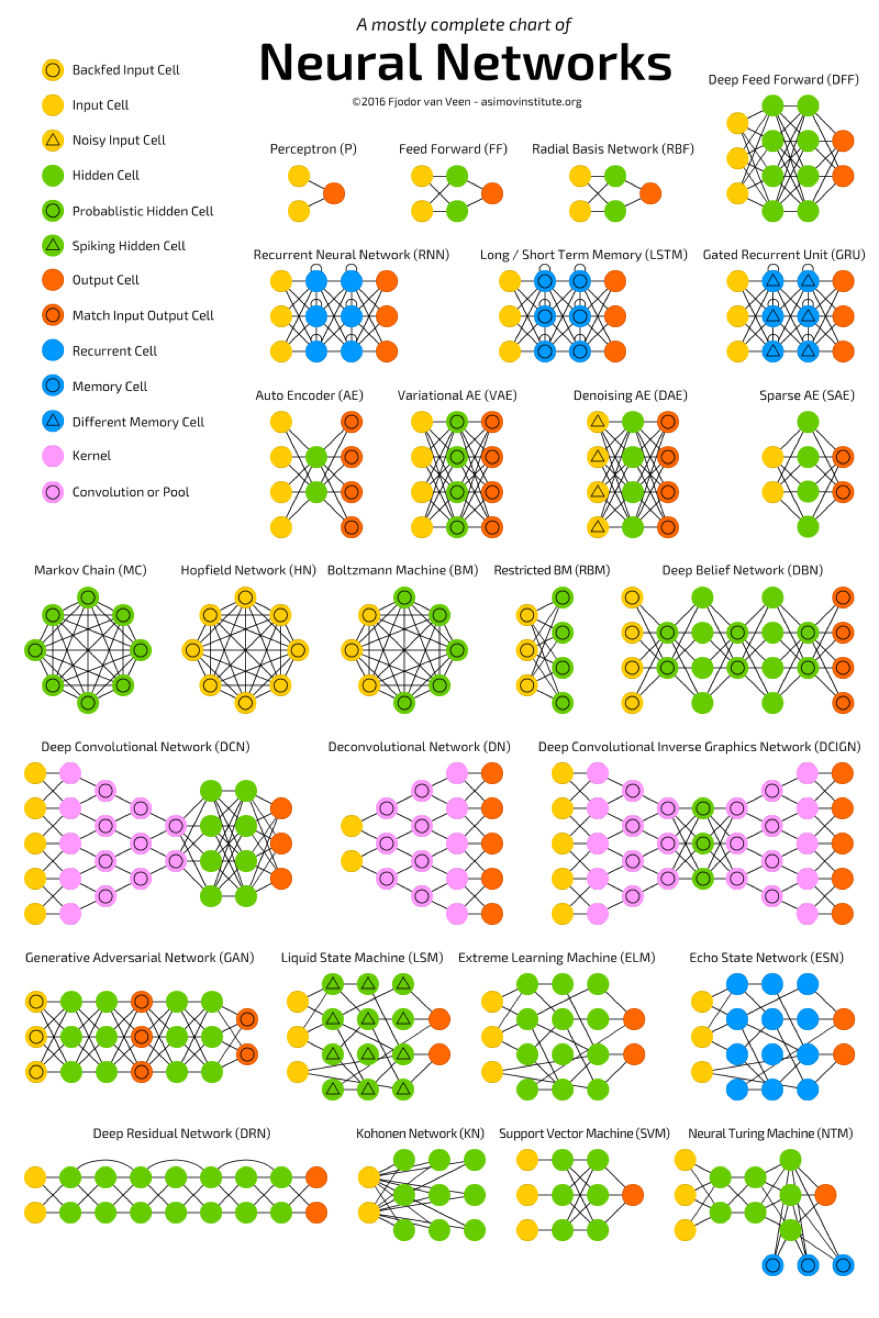
\includegraphics[
        width=\paperwidth,
        height=20cm,
		keepaspectratio]{media/neural-networks}}
	\caption{Neural Network Architectures}
	\label{fig:neural-networks}
\end{figure}

\subsubsection{Deep Auto-Encoder} \label{sec:autoencoder}
% http://on-demand.gputechconf.com/gtc/2017/presentation/s7625-daniel-egloff-going-deeper-in-finance.pdf
An auto-encoder is a DNN that trains the architecture to approximate \textit{X} by itself, i.e. \textit{X=Y}, via a bottleneck structure. This bottleneck layer of the network is where the input features are being reduced, e.g. compressed. This reduction is similar to principal component analysis (PCA) when the auto-encoder is a shallow architecture. Due to the ability to change the number of layers and dimensions, i.e. input units, a deep auto-encoder network (DAE) is much more flexible then PCA. Additionally, DAE introduces nonlinearities in the encoding, whereas PCA can only represent linear transformations.
\begin{figure}[!ht]
	\centering
	\makebox[\textwidth]{
    	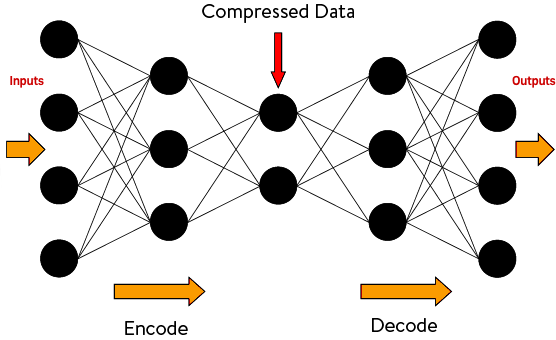
\includegraphics[
        width=\paperwidth,
        height=6cm,
		keepaspectratio]{media/deep-autoencoder-network}}
	\caption{Deep Autoencoder Network Architecture}
	\label{fig:deep-autoencoder-network}
\end{figure}

Figure \ref{fig:deep-autoencoder-network} shows the general architecture of DAE. The network is composed of two symmetrical sides, where one side encodes and the other side decodes, in affect performing a dimensionality and noise reduction. Essentially, a DAE tries to learn to approximate the identity function \ref{eq:autoencoder-approx}.
\begin{equation}
\label{eq:autoencoder-approx}
F_{W,b}\left(X\right) \approx X
\end{equation}
\citet{Takeuchi2013ApplyingStocks} have shown that a DAE can be used to help classify stock momentum. Using momentum input, the DAE is able to discover underlying features by encoding them into the network. The output of the network then provides a classification of a stock being above/below the median of its past return.

The ability for a DAE to encode the features through a reduction will allow us to exploit the high dimensionality of financial trading data.

\subsubsection{Convolutional Neural Network (CNN)} \label{sec:cnn}
% https://towardsdatascience.com/applied-deep-learning-part-4-convolutional-neural-networks-584bc134c1e2
% https://jhui.github.io/2017/03/16/CNN-Convolutional-neural-network/

A CNN is one of the most commonly used architectures. It is primarily used for image recognition, due to its ability to identity the patterns that lead to shape recognition. The convolution refers to the merging of two datasets. In CNNs, an (n x n) matrix, called a filter, is applied to the input matrix. This convolution then results in a feature map.

The use of filters is a common technique used in image processing, which is one of the reasons why CNNs are used in the problem space. When processing an image the filter is applied to the image by sliding along the image, pixel by pixel. The data is passed to the convolution layers, that form a funnel (compressing detected features). This is a similar property as DAE where a compression of features happens in the encoding layers.

The architecture of a CNN can be thought of two core pieces; the first a feature extraction part, and second a classification part. Figure \ref{fig:cnn-architecture} reflects the complete architecture. The first section is the convolution and pooling layers, which are responsible for the feature extraction. When there is a high number of filters being used, then this results in a high dimensional feature map. To reduce the dimensionality in a non-linear manner, pooling is used. A pool is a (n x n) matrix that is applied to the feature map. After the pooling, a fully connected layer performs a classification and assign a probability for each classification.

\citet{Ding2015} demonstrate the use of different variations in the CNN architecture, and how they can be leveraged to perform word embedding to ascertain sentiment of stock events, e.g. news. By using an embedding approach the CNN can then help perform the prediction. Data within time-series data can be expressed in a sliding window manner for analysis. These windows can then be used as embeddings into a CNN.

\begin{figure}[!ht]
	\centering
	\makebox[\textwidth]{
    	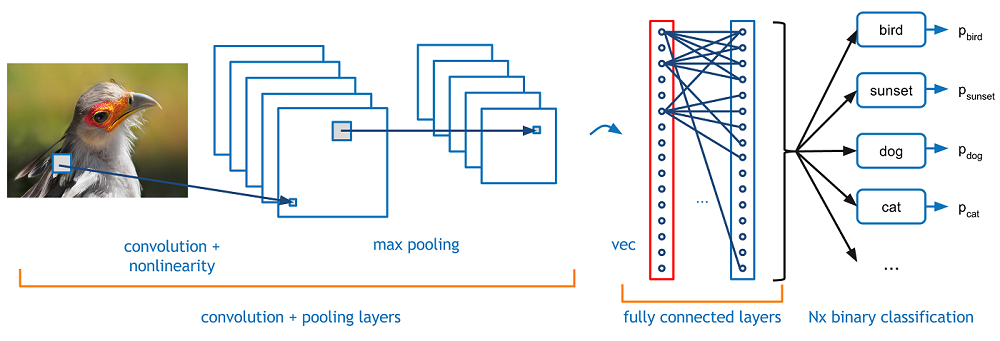
\includegraphics[
        width=\paperwidth,
        height=5cm,
		keepaspectratio]{media/cnn-architecture}}
	\caption{CNN Architecture \cite{A19}}
	\label{fig:cnn-architecture}
\end{figure}

\subsubsection{Recurrent Neural Network} \label{sec:rnn}

RNN is a fully connected network, where each unit is connected to all units in the previous layer. The difference between a DNN, like CNN, and RNN, is that DNNs are stateless between epochs. This means that between transitions the network does not remember the previous outcome \cite{Lipton2015ALearning}. In most cases this is not a concern; however, for problem domains such a language where each word in a sentence makes only sense in the context of what is stated before, state is needed. Specifically, in this domain we are interested in where there is a sequence of events that are indicative of a signal, we need to have state.

To accomplish this a unit, in the hidden layers, has its own output as an input with a fixed delay of one or more epochs. This creates a feedback loop back into a unit, essentially creating state. The way the RNN is built is not different than other DNNs. The unit actually unfolds into multiple units where each unit passes its output \textit{\(h_t\)} to the next unit as shown in Figure \ref{fig:rnn-unrolled}. The input at time \textit{\(x_0\)} is fed into unit \textit{A}, and the activation of \textit{A} is then fed as an input to the next unit and combined with input at time \textit{\(x_1\)}. The difference with RNNs is that the inputs \textit{\(x_0 ... x_t\)} are provided as a sequence to the network. Each unit in the network can be described as an update at epoch \textit{t} to the hidden state \textit{\(h_t\)}, through Equation \ref{eq:rnn-state-update}.

\begin{equation}
\label{eq:rnn-state-update}
h_{\left(t\right)}=f\left(h_{\left(t-1\right)},x_t\right)
\end{equation}

\begin{figure}[!ht]
	\centering
	\makebox[\textwidth]{
    	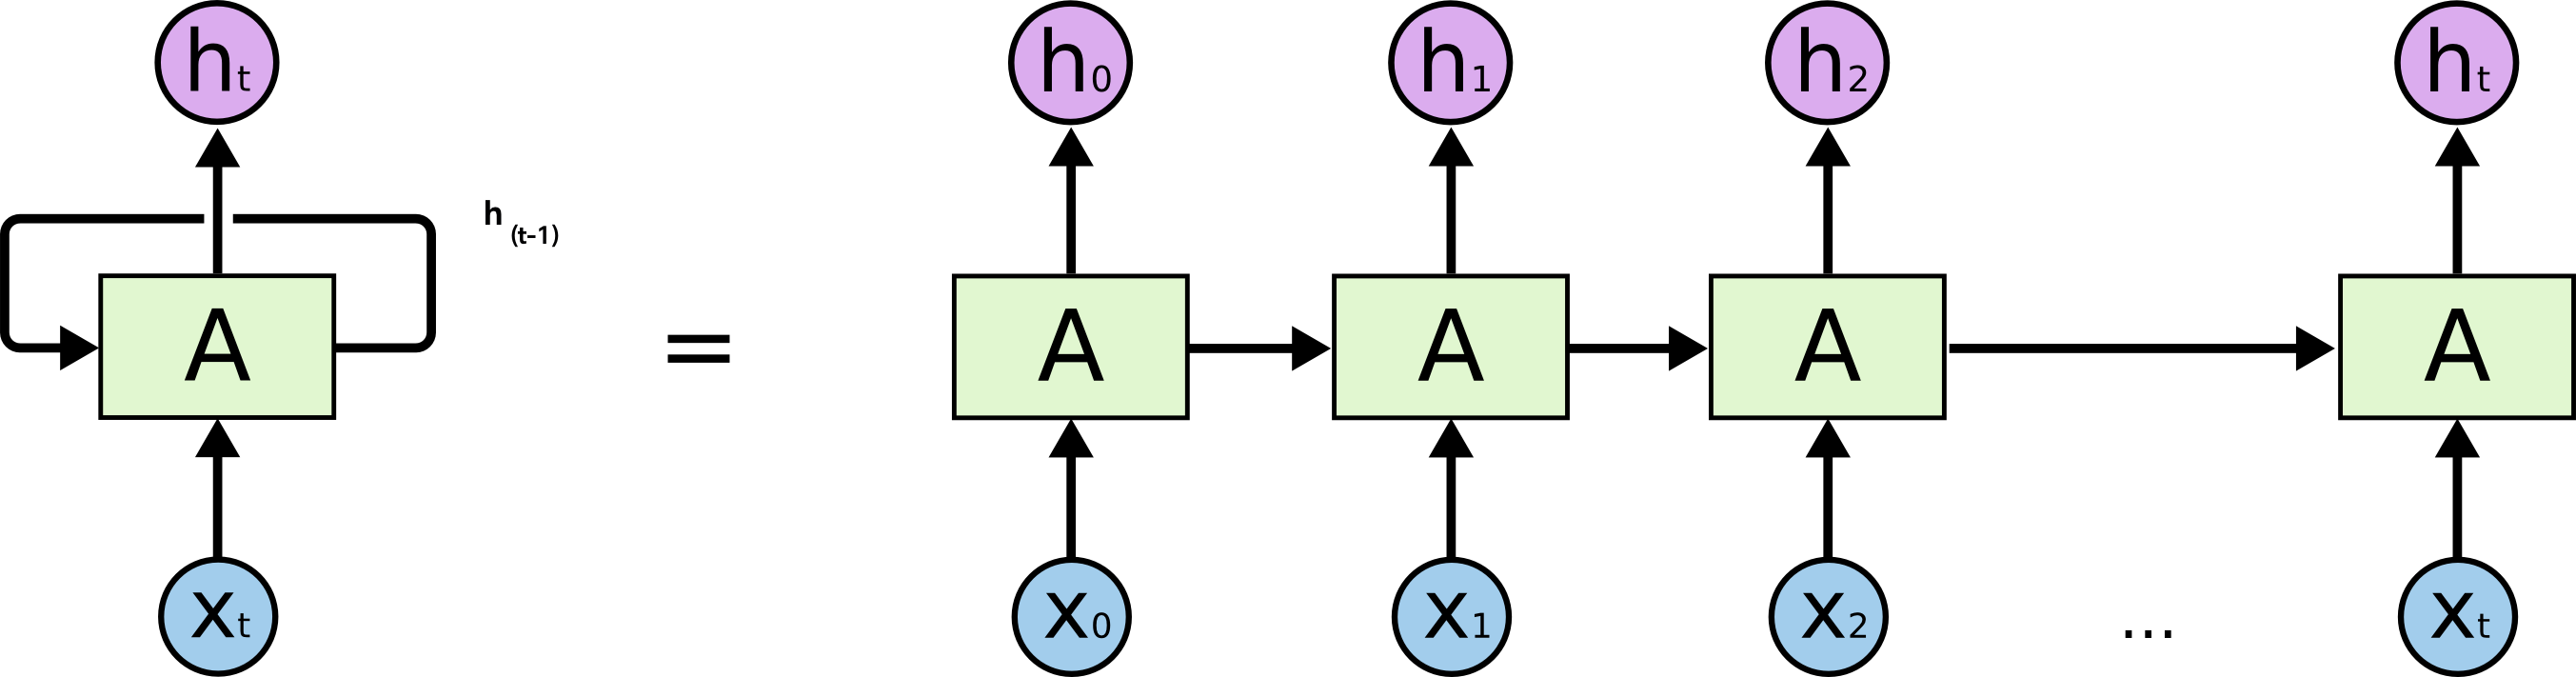
\includegraphics[
        width=\paperwidth,
        height=5cm,
		keepaspectratio]{media/RNN-unrolled}}
	\caption{RNN Expanded\cite{Olah2015UnderstandingBlog}}
	\label{fig:rnn-unrolled}
\end{figure}

\subsubsection{Long Short-Term Memory} \label{sec:lstm}
%http://colah.github.io/posts/2015-08-Understanding-LSTMs/

A described in Section \ref{sec:dnn} backpropagation is used in DNNs to propagate the gradient, and update the weights, through the network. A challenge with back propagation is that if there is a poor local optimum, at any point in the network, then this propagates. This problem is called the vanishing gradient. \citet{Hochreiter1997LONGMEMORY} introduced the LSTM model primarily in order to overcome this problem. Vanishing gradient, or exploding gradient, comes from the use of the chain rule in the backpropagation algorithm. By taking the product of the gradients, it essentially decreases exponentially with the number of layers. This effect has the largest impact in the front of the network and causes its training to be slower.

LSTM is an RNN network, where the activation gates are replaced by a ``memory unit''. Each unit has a cyclical edge with a weight of one. This ensures that the gradient crosses many steps without vanishing or exploding. The specialization in LSTM is that the memory gate is a composite unit build from other gates.

Figure \ref{fig:lstm-chain} describes the gates inside of the ``memory unit''. First, the unit receives the previous memory state \textit{h\textsubscript{\(t-1\)}} and determines if it needs to keep this information using a sigmoid function in the ``forget layer''. Next it will determine what to memorize based on \textit{h\textsubscript{\(t-1\)}} and \textit{\(X_t\)}, and apply a sigmod and tanh function. Finally, the output layer determines the output \textit{h\textsubscript{t}} and sends the output to the next unit.

The term long short-term comes from a DNN network having long-term memory in the form of its weights, and the short-term memory from the units passing information to each other in sequence.

\begin{figure}[!ht]
	\centering
	\makebox[\textwidth]{
    	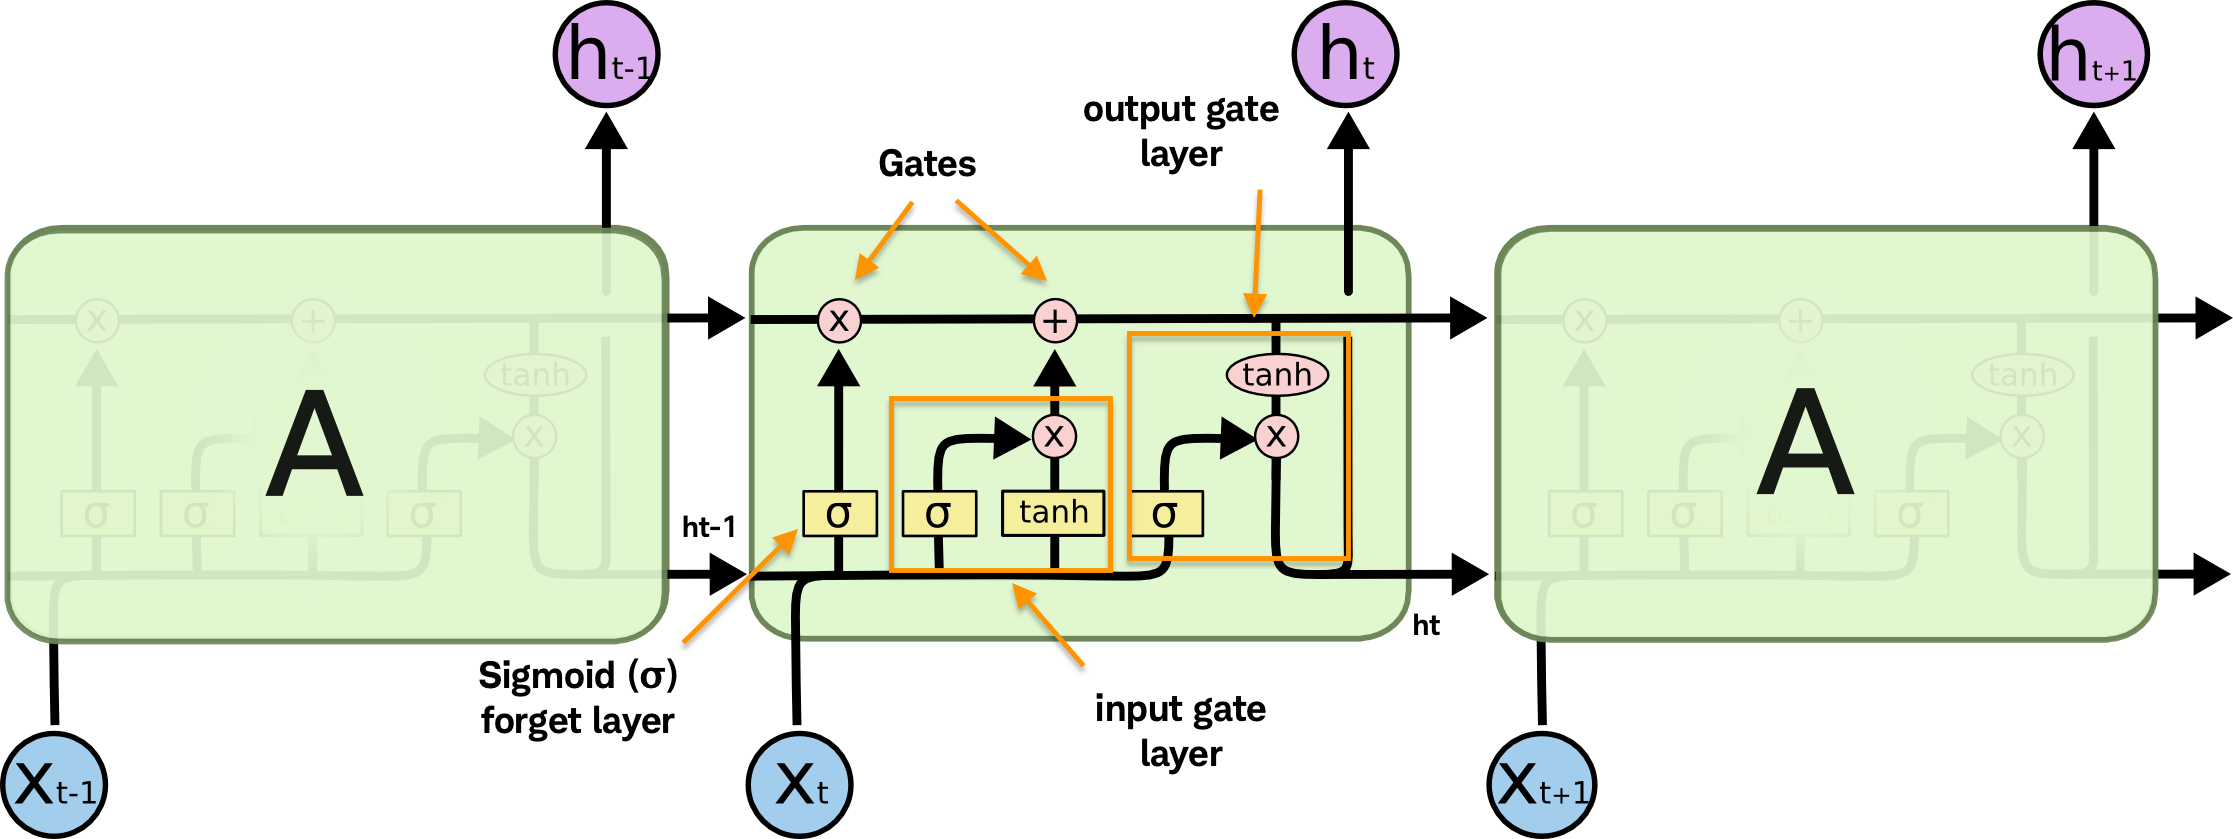
\includegraphics[
        width=\paperwidth,
        height=5cm,
		keepaspectratio]{media/lstm-chain}}
	\caption{View of an LSTM section \cite{Olah2015UnderstandingBlog}}
	\label{fig:lstm-chain}
\end{figure}

\subsubsection{Gated Recurrent Unit} \label{sec:gru}

\citet{ChoLearningTranslation} proposed a gated recurrent unit (GRU) for time-series that allow for different time scales, and simplified calculations. Similar as LSTM's unit, described in Section \ref{sec:lstm}, the unit follows Equation \ref{eq:rnn-state-update}. Where the previous output \textit{h\textsubscript{\(t-1\)}} is fed back into the unit. The simplified part of a GRU is that it does not have the additional gates that form the memory-gate.

Figure \ref{fig:gru-gate} provides a graphical depiction of the unit. The unit has two main gates; gate \textit{z} and \textit{r} which are called the update and reset gates respectively. The update gate determines if the hidden state \textit{h\textsubscript{t}} needs to be updated with the new state. This allows the control of how much information from the previous hidden will be attributed to the current hidden state. This approach allows it to behave like the memory gate in the LSTM network and provides the longterm memory.

To determine if the previous hidden state \textit{h\textsubscript{\(t-1\)}} is to be ignored we have a reset gate. The gate allows the unit to control the information that it deems to be irrelevant in the future, e.g. the next unit. The function of ignoring is similar to compacting a representation, like what encoding performs. Specific comparisons to Encode-Decoding by \citet{ChoOnApproaches} and LSTM by \citet{ChungEmpiricalModeling} have demonstrated that GRU has similar characteristics, with an additional benefit of simplifying the computational aspects. This becomes important later, when needing to scale the architecture, for long sequential problem domains.

\begin{figure}[!ht]
	\centering
	\makebox[\textwidth]{
    	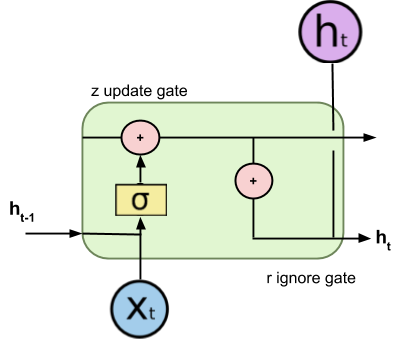
\includegraphics[
        width=\paperwidth,
        height=5cm,
		keepaspectratio]{media/gru-gate}}
	\caption{Gated Recurrent Unit\cite{ChungEmpiricalModeling}}
	\label{fig:gru-gate}
\end{figure}

\subsection{Data Sciences Lab} \label{sec:ds-lab}
As with any sciences, a laboratory allows for a controlled environment in which to perform experiments. A lab environment for a Data Scientist does not have a physical environment in a building, rather a virtual one. When performing experiments a scientist leverages notebooks to help describe the approach, experiments, and findings. In the data sciences community, it is very common to leverage Jupyter Notebooks \cite{JupyterJupyterNotebook} to perform experiments.

Jupyter Notebook is a web application that allows a scientist to author documents that contain code, equations, visualizations, and narrative text. The code that can be placed in the notebook can be different programming languages; however, Python is one of the most prevalent ones. The architecture of a notebook is described in Figure \ref{fig:jupyter-architecture}. A notebook is defined in a notebook file (.ipynb) that can interactively be edited by the user and gets executed by a kernel. The later is specific to the programming language used in the notebook. For the purposes of our experiments, we developed a notebook for each experiment that we ran.

As mentioned previously, Python is one of the most prevalent programming languages in the data sciences community. Part of this reason is the rich set of frameworks that simplify the work needed to implement data munching, data cleansing, plotting, and ML. Core frameworks such as Pandas \cite{McKinneyPythonLibrary} and Scikit Learn \cite{Scikit-learn:Documentation}, have democratized and commoditized the ability to perform experiments. Scikit Learn has provided a wealth of ML algorithms implementations, similarity the Keras \cite{CholletKeras} framework has provided a high-level abstraction to creating DNNs. Keras abstracts the numerical computation libraries Theano and TensorFlow. All the mentioned frameworks are being used during our experiments, with the exception of Theano.

Finally, DNNs can be significantly large graphs and combined with a large amount of data that is necessary to train them, and it creates a significant computational challenge. To solve this computational challenge and allow for massively parallel processing, Google developed Tensorflow \cite{Agarwal2015TensorFlow:Systems}. Tensorflow is a framework for numerical computation for the purpose of ML. It can model classic ML algorithms and DNNs. In fact, it provides framework compatibility with Scikit Learn for easy adoption.

Tensorflow provides a model using directed acyclic graphs (DAG). The DAGs represent the computational graph in a data flow like model, where the framework then can map the computation to different hardware platforms. As such, this allows optimizing around computational power of graphical processing Units (GPU) and tensor processing units (TPU). The later being optimized hardware developed by Google. For our purposes, the details of Tensorflow are abstracted by the Keras framework. Due to Keras leveraging Tensorflow, we are able to exploit Tensorflow's tooling to perform our analysis of the performance of the models. One of those specific tool is TensorBoard, which provides us the visualization of the scalar metrics and insights into the training process.

\begin{figure}[!ht]
	\centering
	\makebox[\textwidth]{
    	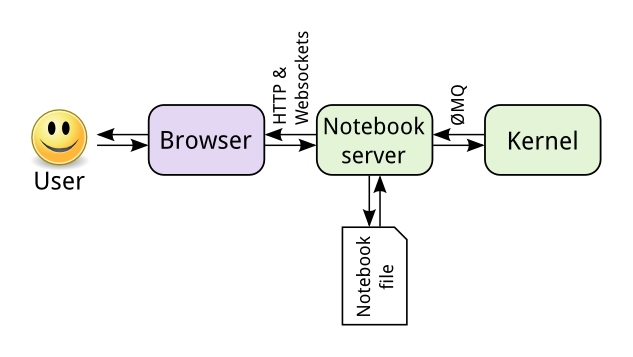
\includegraphics[
        width=\paperwidth,
        height=5cm,
		keepaspectratio]{media/notebook_components}}
	\caption{Jupyter Notebook Architecture}
	\label{fig:jupyter-architecture}
\end{figure}

\section{Experiments} \label{sec:experiments}

As part of the analysis, there are a number of dimensions we wanted to explore. The exploration leads us to try to answer the following questions:
\begin{itemize}
\item How do the different DNN architectures compare with respect to predictive performance?
\item Which architecture computationaly performs best?
\end{itemize}

% \begin{itemize}
% \item How do the different DNN architectures compare with respect to predictive performance?
% \item How well do the architectures perform from a computational perspective?
% \item How does the windowing size impact the performance?
% \end{itemize}

\subsection{Design of the experiments} \label{sec:design-experiments}

This section describes how we designed our experiments, and the data that was leveraged.

The financial dataset that was used for the experiments was that from Quandl \cite{QuandlFinancialQuandl}. It is a source of financial, economic, and alternative datasets, serving investment professionals. The data on the platform is used by industry for different financial analysis, such as hedge funds and asset managers. The platform provides numerous datasets; however, we specifically leveraged the Wiki \textit{EOD Stock Prices} dataset (WIKI/PRICES). The complete dataset contains the end of day (EOD) stock prices, dividends, and splits for 3,000 US companies. The data is curated by the community.

Quandl provides convenient means of accessing the data, either through direct download, or their API. As they provide a Python API, we choose to leverage this approach. By using the API, it allowed us to cache the data locally and refresh when needed. The time-series data covers the time frame from 12-12-1980 till 11-24-2017, which is close to thirtyseven years of daily market data. For our experiments, we will keep it limited to one stock, Apple (APPL), primarily as this stock has had a number of corporate actions. By limiting it to one stock we control for other fundemental changes. Additionally, generalizing a model across stock increases complexity due to fundementals being different, and specific models are needed per security. Each row of data contains a set of features described in Table \ref{tab:features} and the data statistics described in Table \ref{tab:apple-stock-stats}.

\begin{table}[]
\centering
\begin{tabular}{@{}ll@{}}
\toprule
Statistic & Value      \\ \midrule
count     & 9317       \\
mean      & 20.225327  \\
std       & 36.764488  \\
min       & 0.161731   \\
25\%      & 0.918875   \\
50\%      & 1.426153   \\
75\%      & 18.090895  \\
max       & 175.880005 \\ \bottomrule
\end{tabular}
\caption{Apple dataset statistics}
\label{tab:apple-stock-stats}
\end{table}

% https://blog.quandl.com/guide-to-stock-price-calculation
% https://www.investopedia.com/terms/a/adjusted_closing_price.asp
The core time-series data feature is that of the closing price of a security. The closing price represents the market's valuation of the given stock at the end of a trading day. The prices change daily to reflect this valuation and possible corporate actions. Corporate actions are when a company decides to split the stock, or pay a dividend. When this occurs, the stock price will reflect this action. This change in stock prices is not ideal for time-series data analysis.

When an action is taken, such as a split, the price drops to the fraction of the split, which causes noise in the time-series data. These changes in price need to be adjusted for or eliminated from the data. Historical stock prices must be transformed so that the data is indicative of the total return that would have been achieved by holding a particular stock over a particular period of time. As an example, as shown on Figure \ref{fig:adj-vs-close}, Apple's stock seems to drop significantly on June 9th, 2014. This significant drop would impact the ability to perform an analysis.

To accomplish this, the adjusted closing price feature is available. An adjusted closing price is a stock's closing price on any given day of trading that has been amended to include any distributions and corporate actions that occurred at any time prior to the next day's open. The adjusted closing price is more indicative of the performance of a security over time, which is its ``economic reality''. Adjusted stock prices are the foundation for time-series analysis of equity markets.

Stock prices are almost always backward-adjusted. This convention means that in any time series, the stock price for ``today'' matches the current exchange traded price. Historical stock price adjustments are usually multiplicative. This ensures that the returns from holding a stock on non-adjusted days are unchanged by any stock price adjustment. The experiments that we have conducted will leverage the adjusted stock price.

\begin{figure}[!ht]
	\centering
	\makebox[\textwidth]{
    	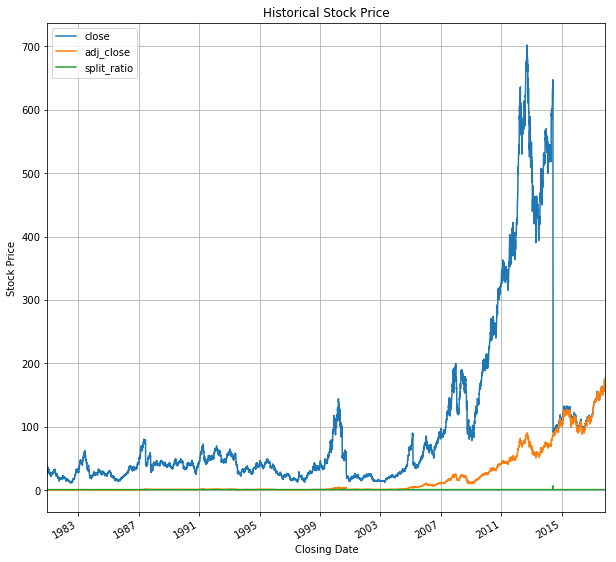
\includegraphics[
        width=\paperwidth,
        height=10cm,
		keepaspectratio]{media/adj-vs-close}}
	\caption{Apple's Closing Price and Adjusted Closing Price}
	\label{fig:adj-vs-close}
\end{figure}

% Daily prediction of a stock price
The goal of the stock prediction is to determine what the valuation of the stock is going to be the next trading day. There are many approaches to perform stock predictions. As pointed out by \citet{Takeuchi2013ApplyingStocks} looking for the momentum trend, they classify if the next day's trend is up or down from today's closing. This is a classification approach. Momentum can be driven primarily by more money moving in and out of the market. For example, a large institution can buy a large amount of shares that can drive up the price. Rather than a classification problem, our predictions will try to predict the next day's price, based on the past price history.

To evaluate the performance of the model we need to establish a measure for comparison. In Section \ref{sec:training} we mentioned that dataset \textit{D} is split in three parts; training, validation, and test. To compare the different architectures we will compare the MAE for the training and validation datasets. Then for the optimized results, we will evaluate the performance of the test data.
% Total 9317
% Train vs. Test (80/20)
% (7403,)
% (1812,)
% mean absolute error (MAE)
% Please add the following required packages to your document preamble:
% \usepackage{booktabs}
\begin{table}[ht]
\centering
% \begin{tabular}{@{}lll@{}}
\begin{tabularx}
% 	{\linewidth}
	{\textwidth}
%     { l l }
% 	{X p{1cm}|>{\raggedright\arraybackslash}X >{\raggedright\arraybackslash}p{3cm}}
%     { X p{1cm} X }
{>{\hsize=.5\hsize}X>{\hsize=1.5\hsize}X}
\toprule
Feature      & Description \\
\midrule
open         & When a market, like the New York Stock Exchange, opens this price represents the valuation of the first trade. \\
high         & The highest price of a trade during the trading day. \\
low          & The lowest price of a trade during the trading day.  \\
close        & The closing price represents the market's valuation of a given security, and the final trading price at the end of a trading day.  \\
volume       & Volume, the number of shares that were traded. The higher the volume can be an indication that money is moving in/out of the security. Large volumes can cause security prices to be impacted.  \\
ex-dividend  & This indicates if this trading date is the ex-dividend date. The ex-dividend is the date by which an investor has the own the security to received the dividend by the recorded data. The ex-dividend date is typically set for two business days prior to the record date. Stock price tend to drop by the amount of dividend on the ex-dividend date, due to capital being transfered from the company to its investors. \\
split\_ratio & A security split is when a corporation decides to increase the number of outstanding shares by dividing each share. By doing a split it reduces the prices of a security. The split ratio specifies how much the ratio is by which the share I dived. For example, a 2:1 ration means an investor will receive 2 shares for each shared owned. As a result the share price is divided by 2 as well.     \\
adj\_open    & Opening price adjusted for any corporate actions.   \\
adj\_high    & Highest price for the trading day, adjusted for any corporate actions. \\
adj\_low     & Lowest price for the trading day, adjusted for any corporate actions.   \\
adj\_close   & Closing price for the trading day, adjusted for any corporate actions.   \\
adj\_volume  & Volume for the day, adjusted for any corporate actions.  \\
\bottomrule
\end{tabularx}
\caption{Quandl Stock Data Features}
\label{tab:features}
\end{table}

% Window prediction of momentum
\subsection{Time-Series Embedding} \label{sec:embedding}
% http://on-demand.gputechconf.com/gtc/2017/presentation/s7625-daniel-egloff-going-deeper-in-finance.pdf

We use a time-series embedding approach to create a multi-dimensional sequential feature set to train our models under evaluation. The embedding spans multiple epochs in the past. When working with time-series for predicting, a good number of epochs of historical data is needed to ensure the models recognize patterns in the data. Using only one epoch, i.e. last day's price, is not enough data for training. The models will only pick up on the one price.

Figure \ref{fig:time-series-embedding} describes how we will be creating the embedding. For each time event \textit{t}, we will create a lookback window of 50 epochs, which is called the window size. Each window is then a single embedding, which the stock value at \textit{t}.

To ensure that the optimization process in the model can converge to good optimum, we will normalize the data for each embedding, using Min-Max scaling. Each price will be normalized between (min=0, max=1), using the Equation \ref{eq:min-max-function}.
% This will ensure that for each window all data points have a mean of zero (\(\mu=0\)) and a standard deviation of 1 (\(\sigma=1\))).

\begin{equation}
\label{eq:min-max-function}
X_{norm}=\frac{X\ -\ X_{\min}}{X_{\max}-X_{\min}}
\end{equation}

\begin{figure}[!ht]
	\centering
	\makebox[\textwidth]{
    	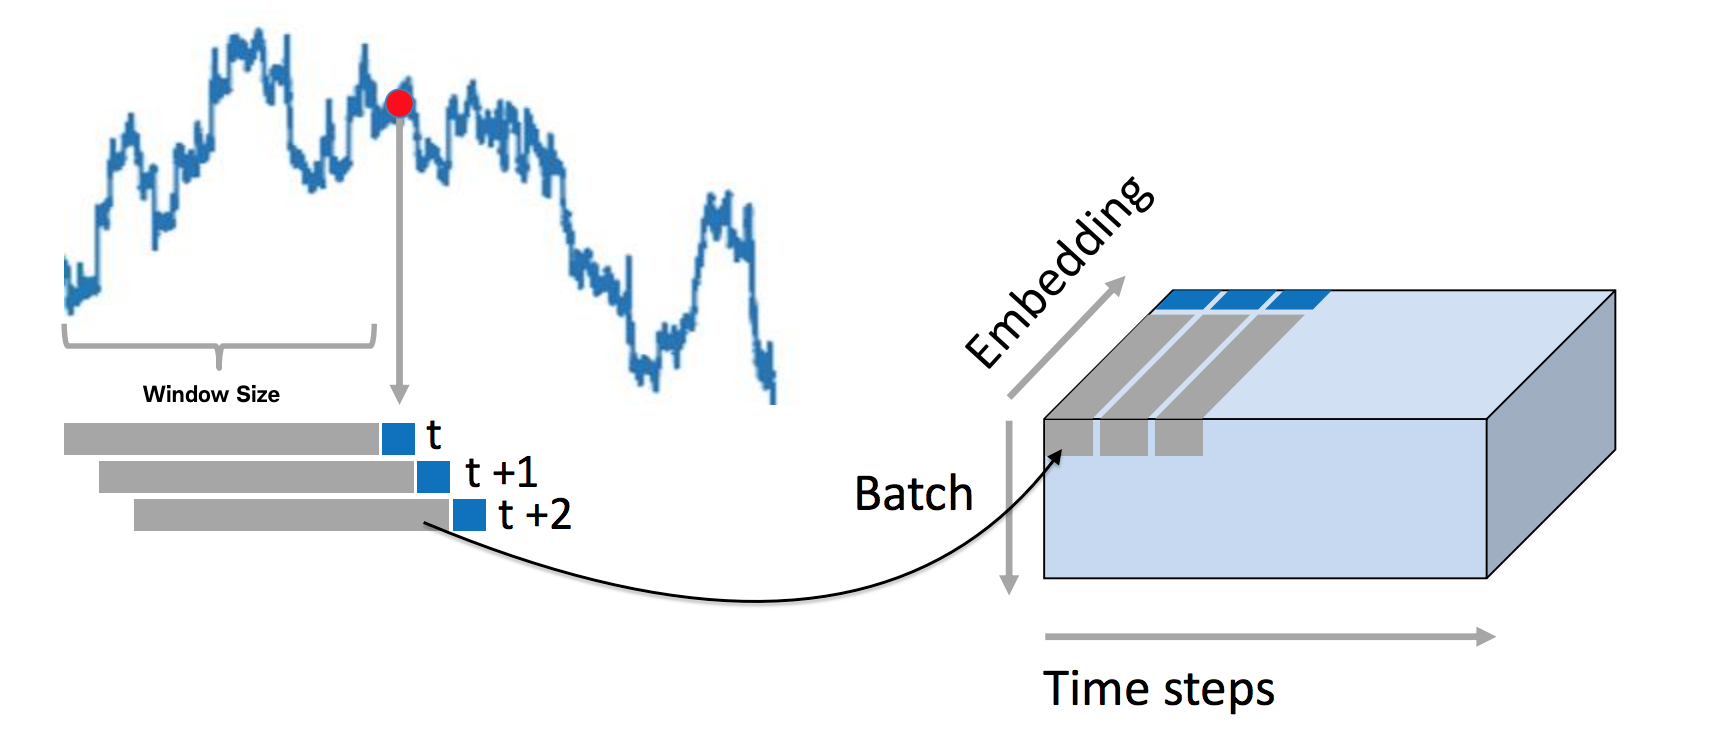
\includegraphics[
        width=\paperwidth,
        height=10cm,
		keepaspectratio]{media/time-series-embedding}}
	\caption{Time Series Embedding}
	\label{fig:time-series-embedding}
\end{figure}


\subsection{Network Topology} \label{sec:network-topology}

For each evaluation, we train each of the architectures using their specific units. Each architecture will have a specific network topology. The topology defines the number of layers and units per layer. Figure \ref{fig:network-architecture} provides a visual representation of all the architectures. We intentionally made the topology relatively small to avoid overfitting and reduce computational time. Table \ref{tab:topology} provides a summary of the topology.

In Section \ref{sec:cnn} we described the common pattern of convolution, pooling, and fully connected layers. For the convolution layers, we will apply 4 filters to produce the filter map. The CNN is shown in Figure \ref{fig:cnn-architecture}.
DAE is a constraining network as described in Section \ref{sec:autoencoder}. The encoding part will take the lookback size of 50 and then constrain it to 7. The decoding part will only bring it to 1 for the single value prediction.
The LSTM, RNN, and GRU are different types of recurrent networks. To keep the experiments comparable, we constrain all three of them to a comparable topology. With each of them, we add dropout layers to prevent overfitting.

% \begin{itemize}
% \item 50 units Convolution Layer as the input using 1 dimensional
% \item 25 units Pooling Layer to perform a reduction
% \item 25 units Convolution Layer as and additional means to find higher order features
% \item 12 units Pooling Layer
% \item 1 unit output layer to perform the final prediction
% \end{itemize}

\begin{table}[]
\centering
\begin{tabular}{@{}llll@{}}
\toprule
ANN  & Topology    & Total \# Of Units & \# of Parameters \\ \midrule
CNN  & 50-25-25-12-1 & 113             & 77               \\
RNN  & 50-25-1     & 76                & 4,526            \\
LSTM & 50-25-1    & 76               & 18,026          \\
GRU  & 50-25-1     & 76                & 13,526           \\
DAE  & 50-14-7-7-1 & 79                & 540              \\ \bottomrule
\end{tabular}
\caption{The topology of the architecture used in the experiments.}
\label{tab:topology}
\end{table}

\begin{figure}
    \centering
    \begin{subfigure}[b]{0.3\textwidth}
        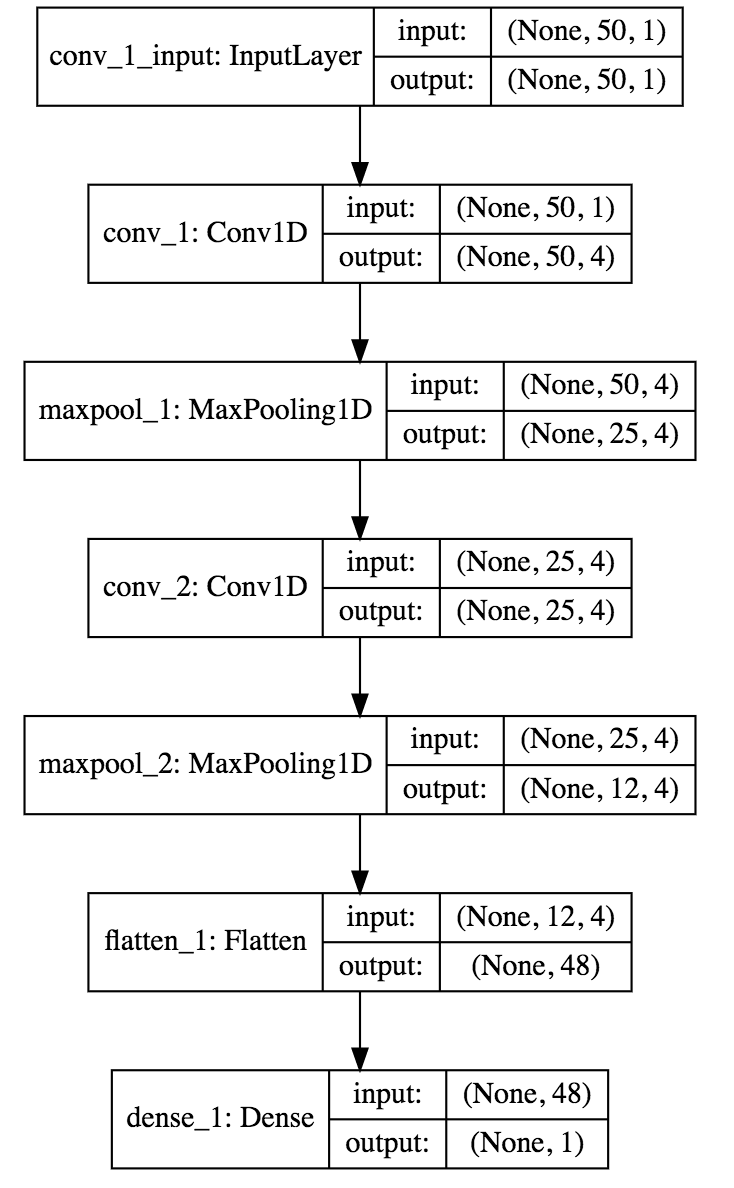
\includegraphics[width=\textwidth]{media/cnn-network}
        \caption{CNN}
        \label{fig:cnn-architecture}
    \end{subfigure}
    ~ %add desired spacing between images, e. g. ~, \quad, \qquad, \hfill etc.
      %(or a blank line to force the subfigure onto a new line)
    \begin{subfigure}[b]{0.3\textwidth}
        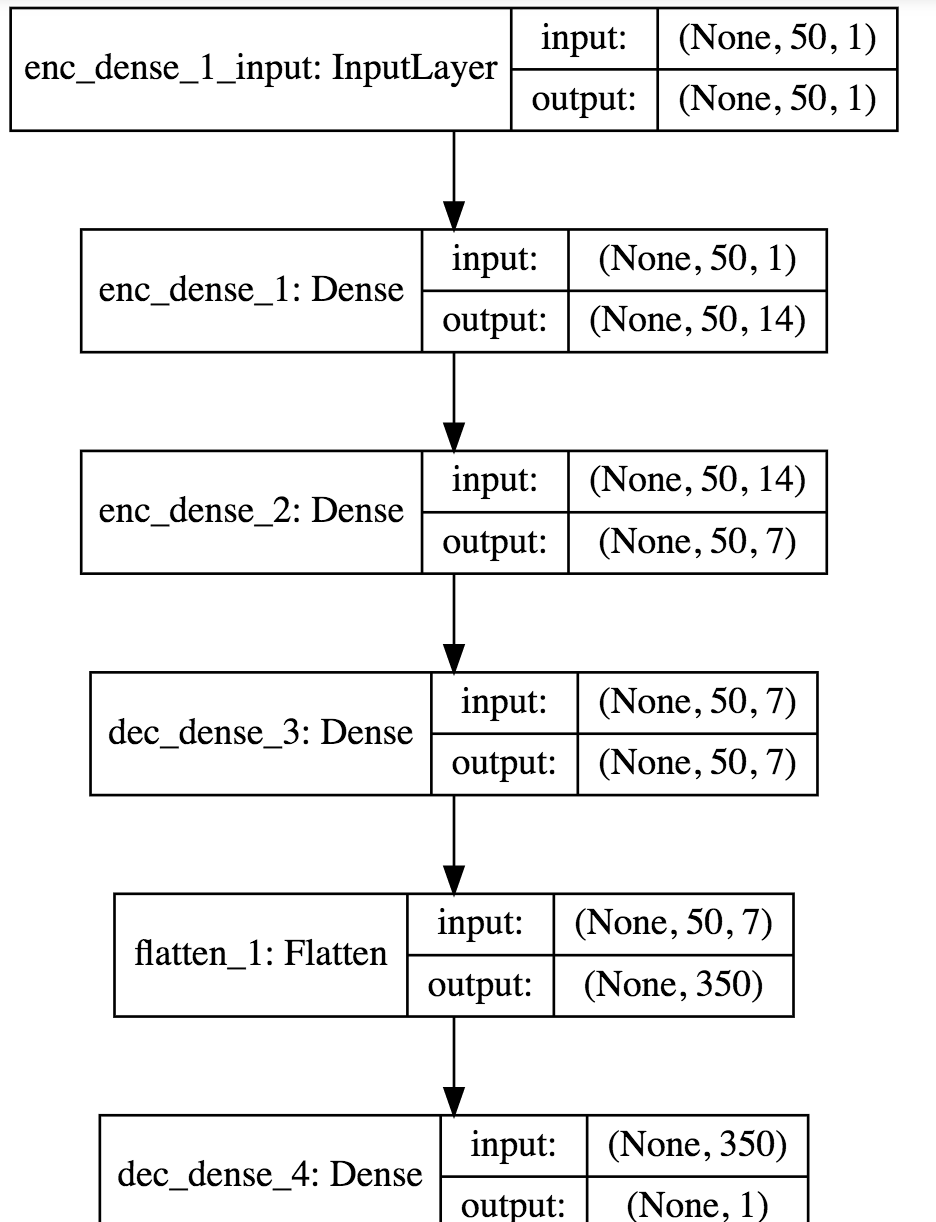
\includegraphics[width=\textwidth]{media/autoenc-network}
        \caption{Deep Auto Encoding}
        \label{fig:autoenc-network}
    \end{subfigure}
    ~ %add desired spacing between images, e. g. ~, \quad, \qquad, \hfill etc.
    %(or a blank line to force the subfigure onto a new line)
    \begin{subfigure}[b]{0.3\textwidth}
        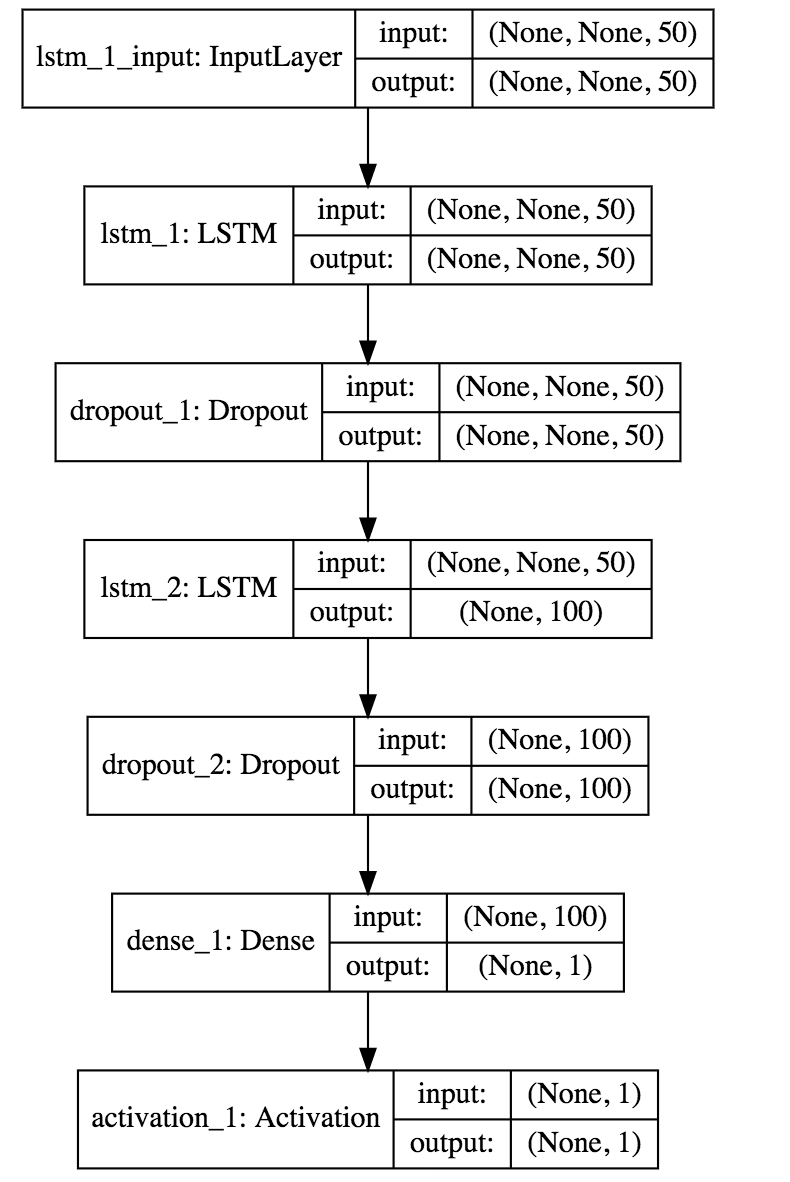
\includegraphics[width=\textwidth]{media/lstm-network}
        \caption{LSTM}
        \label{fig:lstm-network}
    \end{subfigure}
    ~ %add desired spacing between images, e. g. ~, \quad, \qquad, \hfill etc.
    %(or a blank line to force the subfigure onto a new line)
    \begin{subfigure}[b]{0.3\textwidth}
        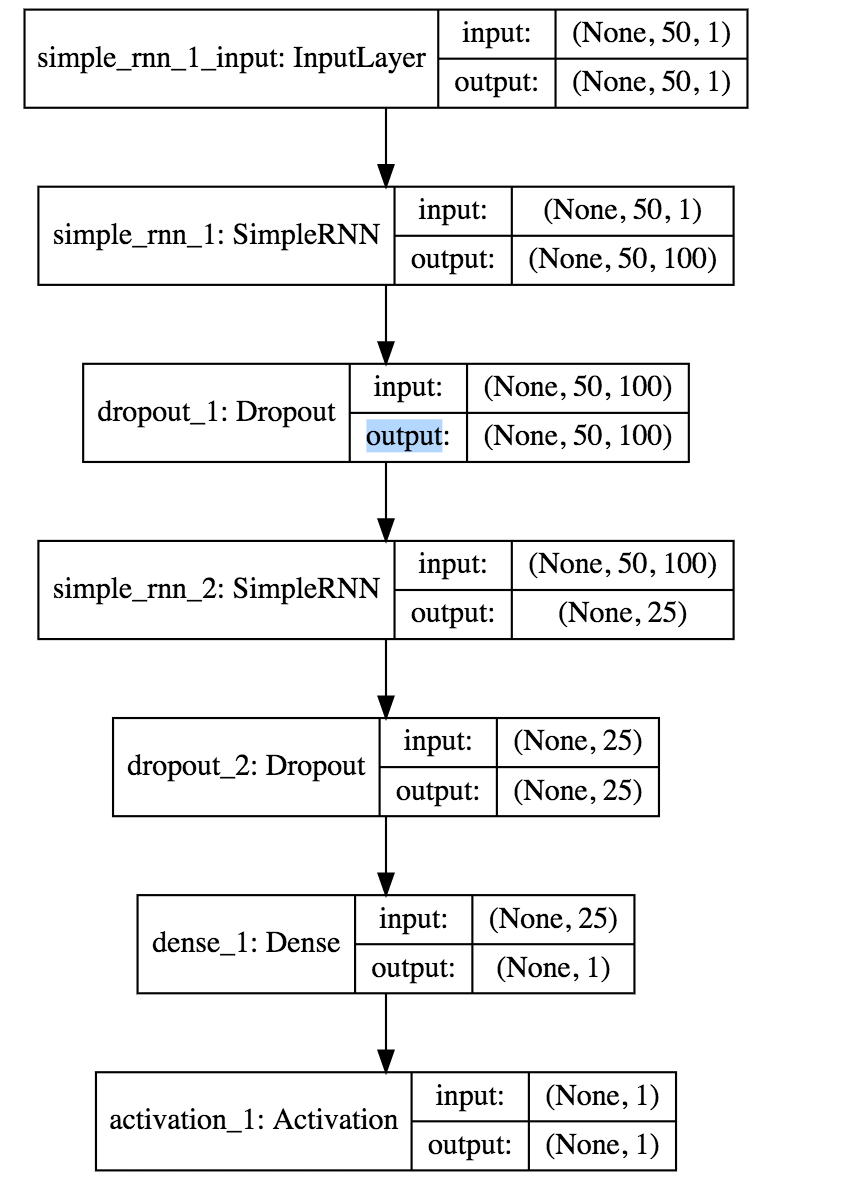
\includegraphics[width=\textwidth]{media/rnn-network}
        \caption{RNN}
        \label{fig:rnn-network}
    \end{subfigure}
    ~ %add desired spacing between images, e. g. ~, \quad, \qquad, \hfill etc.
    %(or a blank line to force the subfigure onto a new line)
    \begin{subfigure}[b]{0.3\textwidth}
        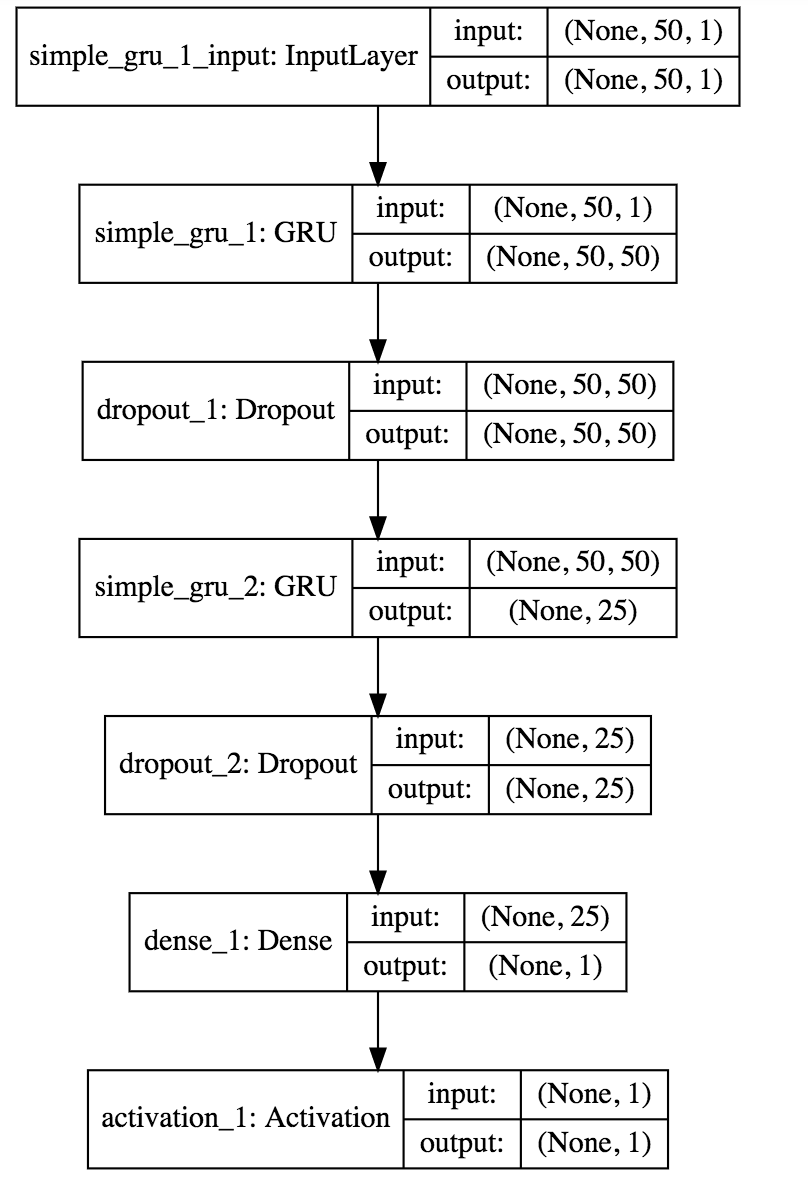
\includegraphics[width=\textwidth]{media/gru-network}
        \caption{GRU}
        \label{fig:gru-network}
    \end{subfigure}
    \caption{Network Architectures and Topology}\label{fig:network-architecture}
\end{figure}

\subsection{Results and Analysis} \label{sec:results}

% \begin{itemize}
% \item How do the different DNN architectures compare with respect to predictive performance?
% \item How well do the architectures perform from a computational perspective?
% \item How does the windowing size impact the performance?
% \end{itemize}

The main results of each experiment is provided in Table \ref{tab:mae-results}. With the main performance metric being MAE, it is clear that GRU outperformed all the others based on the testing data performance. Its performance for the training data is below that of RNN, and LSTM respectively. To make a good model it is important that it generalizes and performs best on real test data. This indicates that GRU does not have a perfect fit for the training data.

\begin{table}[]
\centering
\begin{tabular}{@{}lll@{}}
\toprule
Experiment & Train MAE   & Test MAE    \\ \midrule
LSTM       & 0.002509666 & 0.054925341 \\
CNN        & 0.021865675 & 0.481374076 \\
AEC        & 0.005272924 & 0.159446251 \\
RNN        & \textbf{0.001573065} & 0.071079882 \\
GRU        & 0.003662259 & \textbf{0.010395636} \\ \bottomrule
\end{tabular}
\caption{Performs of each architecture, by showing the MAE for the training data and the testing data. The numbers in bold represent the minimum number in that category, e.g. best performance. }
\label{tab:mae-results}
\end{table}

Another measure of performance is the computational performance of a model. If the prediction performance is comparable to each other, then a model that converges faster on the loss will be ideal. In the FI, being able to run training on a large dataset in the smallest amount of time is a significant benefit. To determine the better performer we need to look how fast (wall time) the model completes. Figure \ref{fig:cpu-loss-performance} shows that RNN is the fastest performer, followed by LST and GRU respectively. Intuitively it makes sense that RNN performs better than architectures with more complex units.

During the experiments, we did not stop the training if we noticed that the gradient for the loss was stabilizing. With many ML frameworks, you can stop training if this is occurring. If we then assume we stop training, then the makespan for the experiments would be different. Looking at Figure \ref{fig:cpu-loss-performance} we notice that GRU performs faster then LSTM. The gates in a GRU are simpler then LSTM, which explains why GRU would perform better. RNN still performs faster; however, its loss is higher then GRU. For this reason, we determine that GRU is a better performer, given the computational and loss performance.

% \begin{figure}[!ht]
% 	\centering
% 	\makebox[\textwidth]{
%     	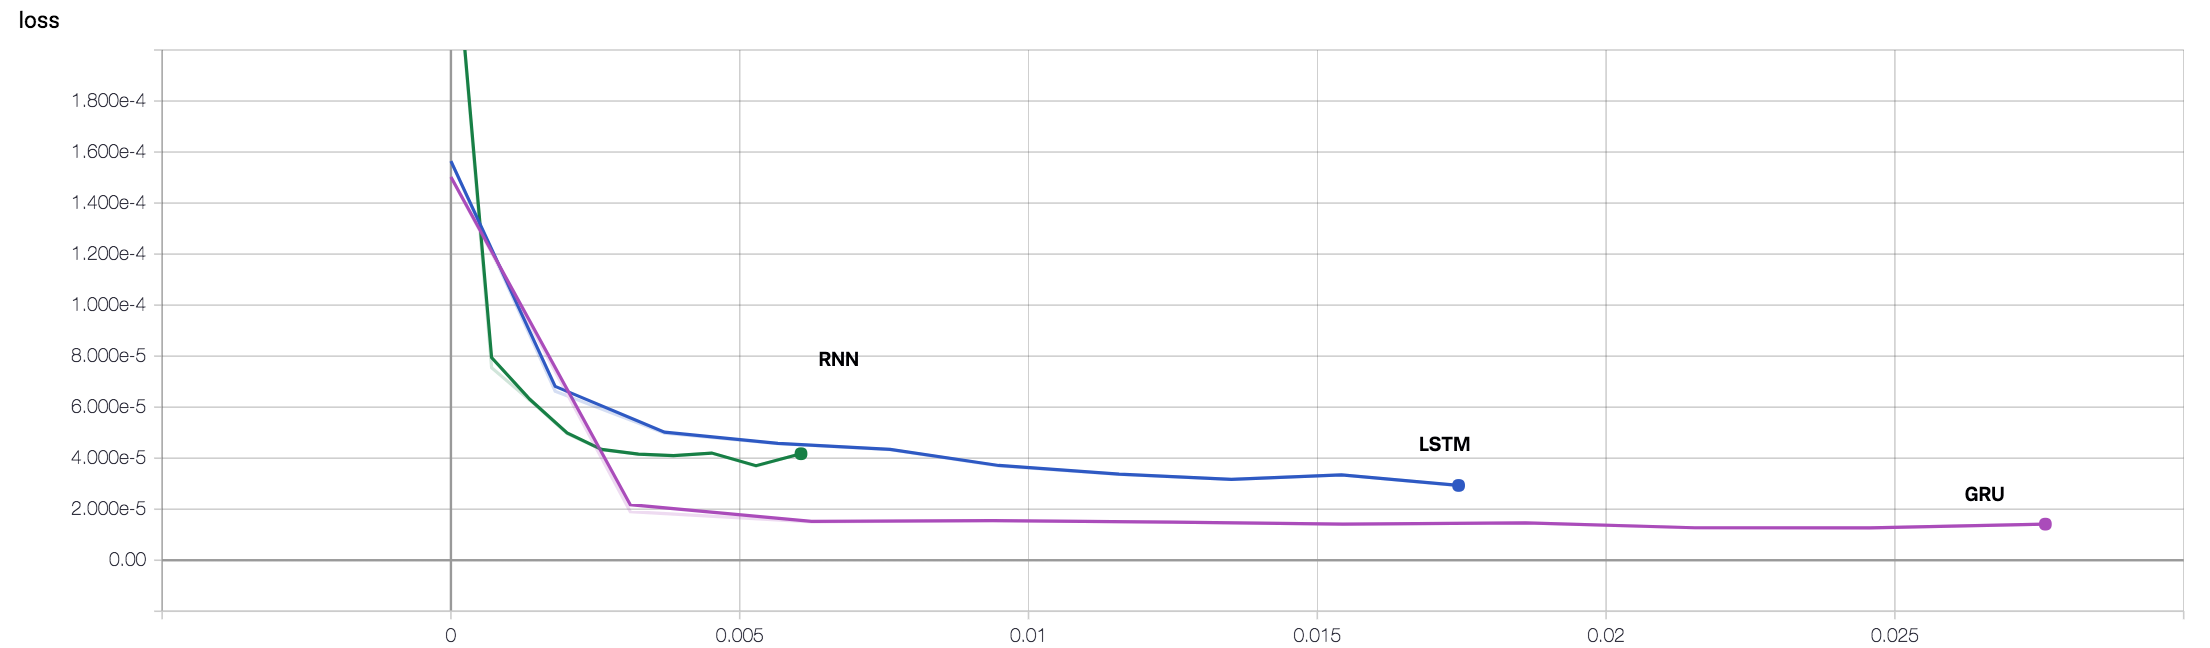
\includegraphics[
%         width=\paperwidth,
%         height=6cm,
% 		keepaspectratio]{media/cpu-loss-performance}}
% 	\caption{For each architecture we show the loss (y-axis) and relative time (x-axis) in seconds.}
% 	\label{fig:cpu-loss-performance}
% \end{figure}

\begin{figure}
    \centering
    \begin{subfigure}[b]{1\textwidth}
        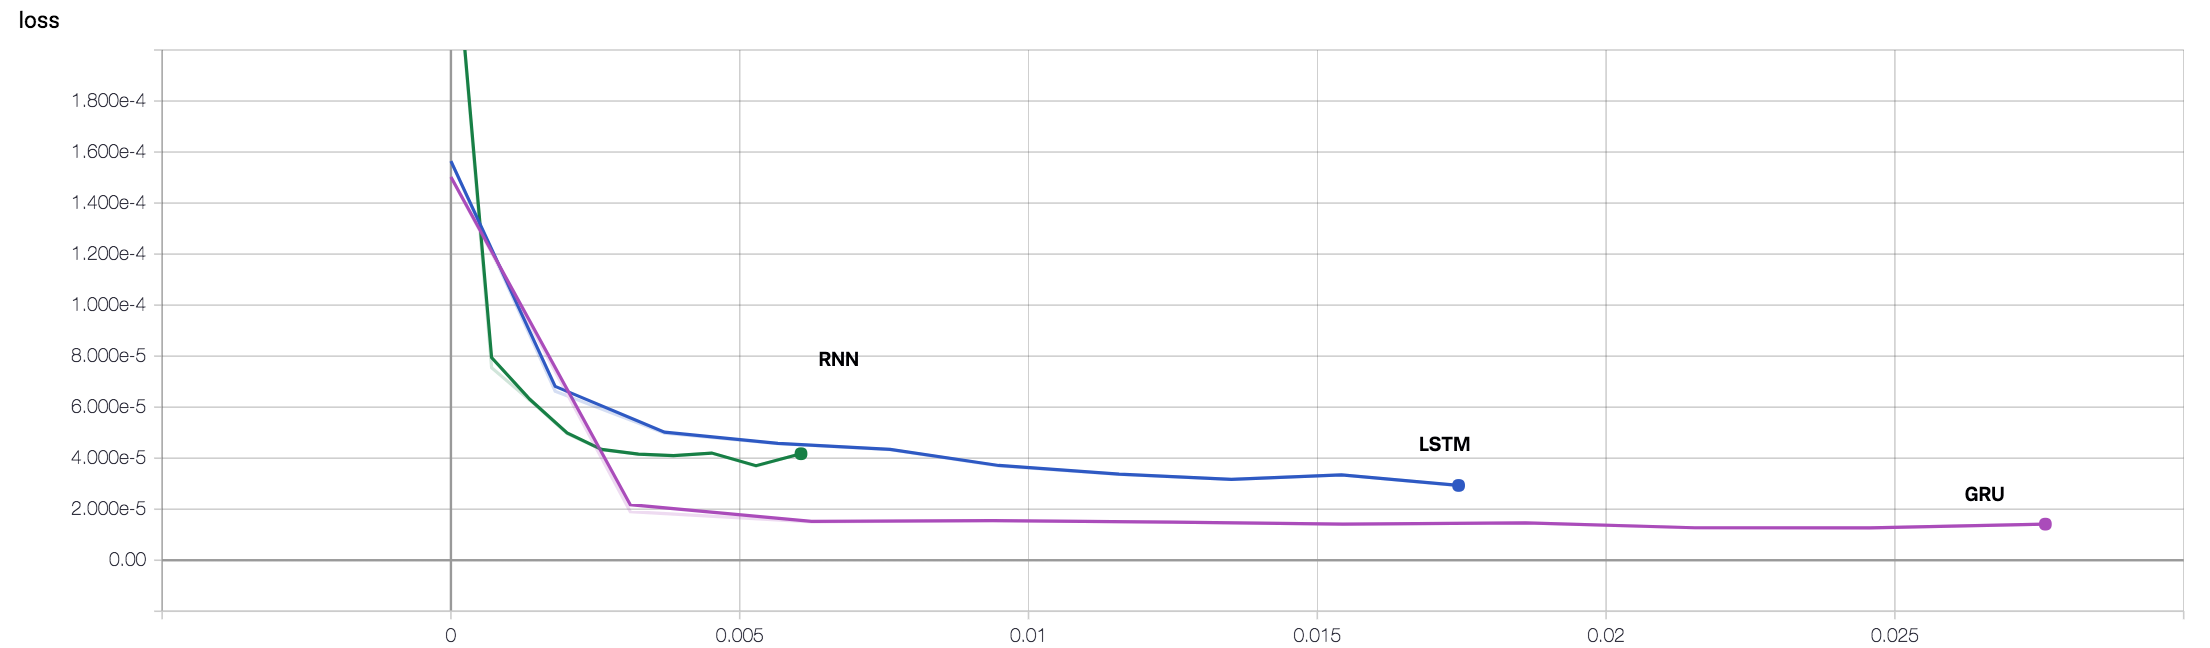
\includegraphics[width=\textwidth]{media/cpu-loss-performance}
        \caption{RNN, LST, and GRU architectures}
        \label{fig:cpu-loss-rnns}
    \end{subfigure}
    ~ %add desired spacing between images, e. g. ~, \quad, \qquad, \hfill etc.
      %(or a blank line to force the subfigure onto a new line)
    \begin{subfigure}[b]{1\textwidth}
        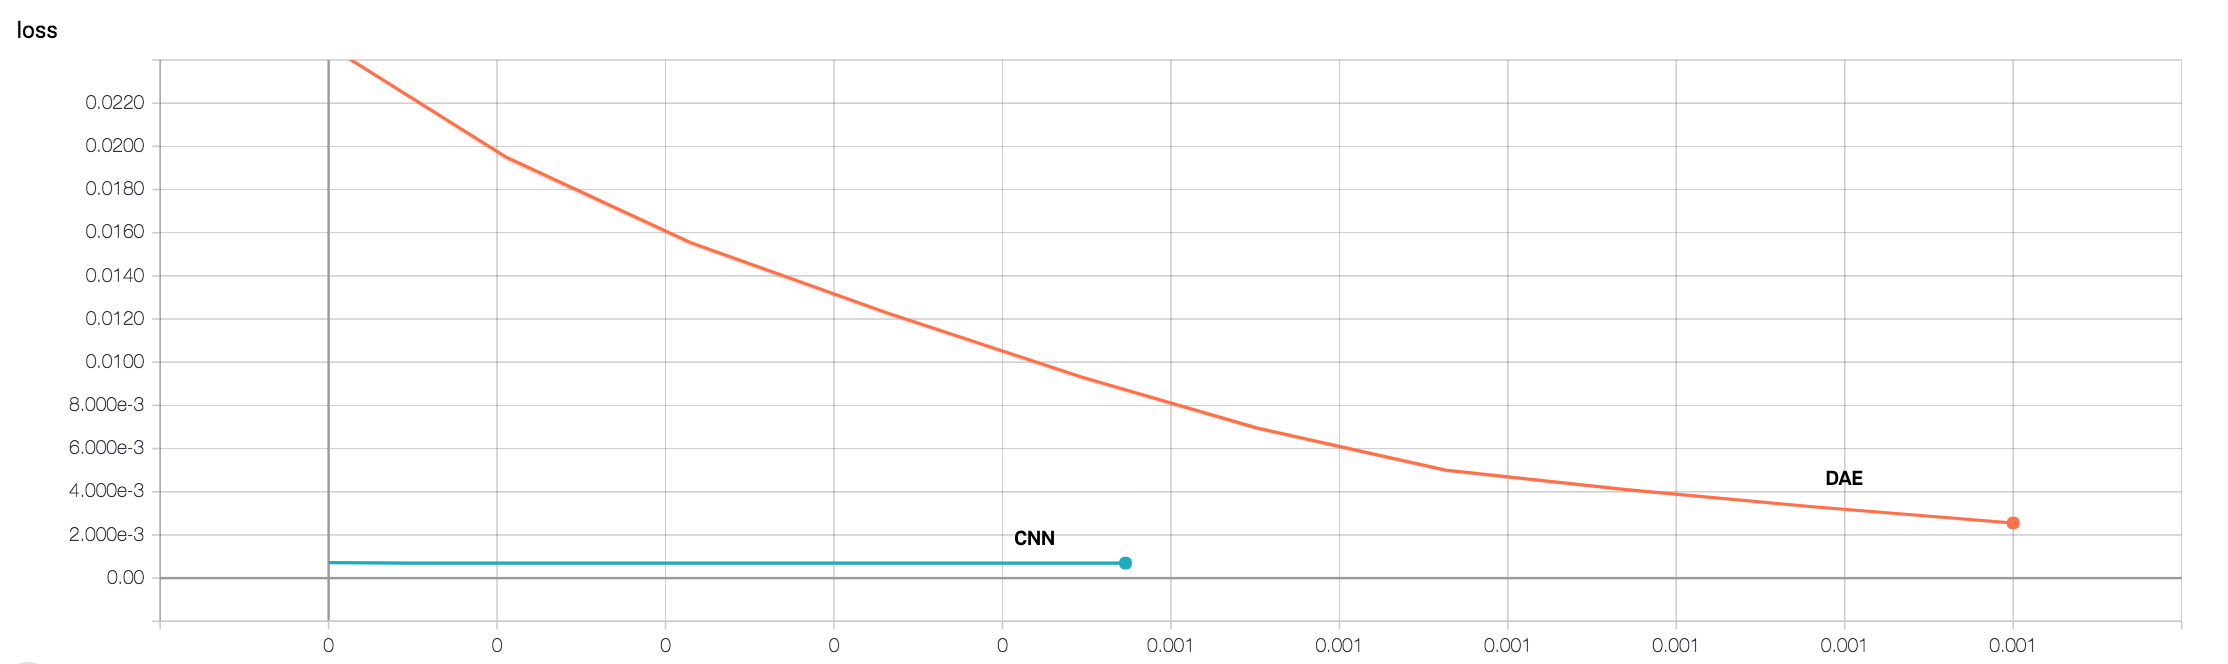
\includegraphics[width=\textwidth]{media/cpu-loss-performance-other}
        \caption{CNN and DAE architectures}
        \label{fig:cpu-loss-others}
    \end{subfigure}
    \caption{For each architecture we show the loss (y-axis) and relative time (x-axis) in seconds. The RNN type architectures are separated from the others as their loss is significantly higher.}
    \label{fig:cpu-loss-performance}
\end{figure}

When we review the actual stock predicting and graph this, as shown in Figure \ref{fig:stock-performance-architecture}, we can see how the predictions are working. The graph displays a prediction that is made for each test data point. As mentioned earlier, the MAE for the RNN type of architectures is the best. As shown in Figure \ref{fig:result-cnn} the CNN is able to closer match at the tail end. On the other hand, DAE's encoding is not able to match close and has a large spread. Due to the hierachal structure of DAE, it is unable to learn the sequential order of the data. This is supported by \citet{ChoOnApproaches} and suggests that a memory gate is better equiped in this case.

\begin{figure}
    \centering
    \begin{subfigure}[b]{0.3\textwidth}
        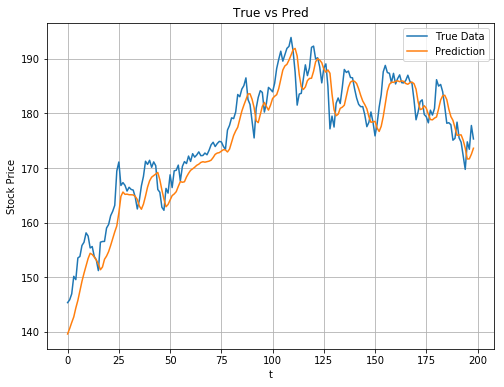
\includegraphics[width=\textwidth]{media/result-rnn}
        \caption{RNN}
        \label{fig:result-rnn}
    \end{subfigure}
    ~ %add desired spacing between images, e. g. ~, \quad, \qquad, \hfill etc.
      %(or a blank line to force the subfigure onto a new line)
    \begin{subfigure}[b]{0.3\textwidth}
        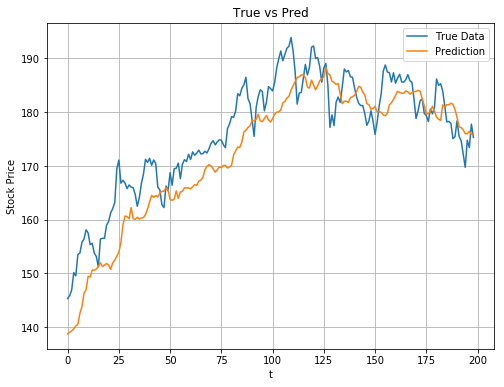
\includegraphics[width=\textwidth]{media/result-cnn}
        \caption{CNN}
        \label{fig:result-cnn}
    \end{subfigure}
    ~ %add desired spacing between images, e. g. ~, \quad, \qquad, \hfill etc.
    %(or a blank line to force the subfigure onto a new line)
    \begin{subfigure}[b]{0.3\textwidth}
        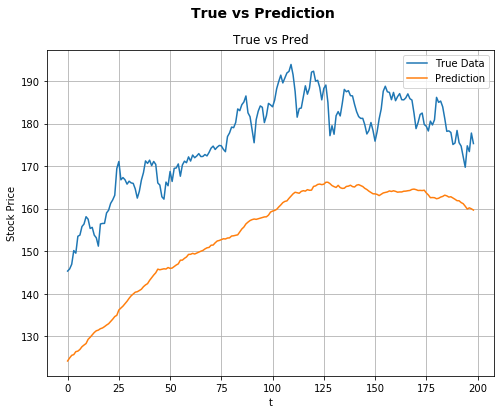
\includegraphics[width=\textwidth]{media/result-dae}
        \caption{DAE}
        \label{fig:result-dae}
    \end{subfigure}
    ~ %add desired spacing between images, e. g. ~, \quad, \qquad, \hfill etc.
    %(or a blank line to force the subfigure onto a new line)
    \begin{subfigure}[b]{0.3\textwidth}
        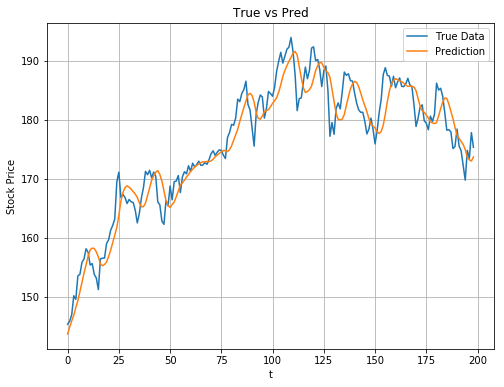
\includegraphics[width=\textwidth]{media/result-lstm}
        \caption{LSTM}
        \label{fig:result-lstm}
    \end{subfigure}
    ~ %add desired spacing between images, e. g. ~, \quad, \qquad, \hfill etc.
    %(or a blank line to force the subfigure onto a new line)
    \begin{subfigure}[b]{0.3\textwidth}
        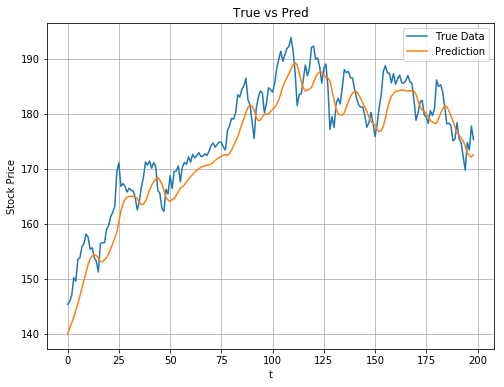
\includegraphics[width=\textwidth]{media/result-gru}
        \caption{GRU}
        \label{fig:result-gru}
    \end{subfigure}
    \caption{Stock price graph showing the True data (test data) compared to the predicted data. The prediction is one at each time step (x) given the last sequence of true data, in effect only predicting 1 step ahead each time.
}\label{fig:stock-performance-architecture}
\end{figure}

\section{Conclusion and Future Work} \label{sec:conclusion}

In this paper we evaluated artificial neural network (ANN) architectures; (1) a recurrent neural network (RNN), (2) long short-term memory (LSTM), (3) gated recurrent unit (GRU), (4) deep auto encoder (DAE), and (5) one of the most popular once convolutional neural network (CNN). Our evaluation focused on using high dimensional financial time-series data. This data is modeled as sequential data while using loopback windows as a feature embedding to the models.

The evaluation clearly demonstrated the superiority of the GRU architecture. This was evident in the prediction performance and computational performance when we considered stopping learning when loss plateaus.

We consider the experiments and results as guidance for specific financial industry time-series problem domains. Specifically, we demonstrated that for basic stock price time-series this can be used. Given the many factors involved in determining a stock price we are convinced that GRU can aid in the analysis; however, additional embedding of events would still be required. We referenced other research that indicates that technicals such as momentum will need to be considered.

Future work can be derived from this work by modeling time-series data as a symbolic representation as described by \citet{Lin2003AAlgorithms} (SAX). This would accomplish the embedding and encoding shown in the architectures we have presented here. What SAX provides is a further ability to use pattern matching, and reducing the time-series data space. In future work we will try to exploit this capability.

% Need to use abbrvnat to make natbib and citealt to work
\bibliographystyle{abbrvnat}
%\bibliographystyle{acm}
\bibliography{Mendeley.bib}
\end{document}
